\newpage
\section*{List of tables and figures}
\addcontentsline{toc}{section}{List of tables and figures}
\listoftables
\listoffigures



\newpage
\section*{Appendix}
Every table and graph in this thesis, the R code that generated them, and the Latex source code of this manuscript are available in the GitHub repository of this project at \url{https://github.com/martin-kosiik/Geopolitics-of-Repressions}.
%To reproduce the analysis, you will need to download the 
If you have any troubles with replications or any other questions, please email me at \href{mailto:martin.kosiik@gmail.com}{martin.kosiik@gmail.com}.
\addcontentsline{toc}{section}{Appendix}
\setcounter{table}{0}
\renewcommand{\thetable}{A\arabic{table}}

\setcounter{figure}{0}
\renewcommand{\thefigure}{A\arabic{figure}}

\subsection*{International Relations Controls}
The summary of major changes in international relations of the Soviet Union with states that have significant minorities in the USSR that we use as control variable in our default  difference-in-differences specification (equation \ref{eq:dynamic_did}) are provided in the table \ref{tab:geopol_relations}. In particular, we created a separate dummy variable for every combination of state and  phase of geopolitical relations. 
The blank cells indicate that no special dummy variable covers that years (i.e. there was no significant change in relations with the given country in that year).
For example in case of Hungarian ethnicity, we created one dummy variable for the period of war with the USSR (from 1941 to 1944) and another one covering the whole post-1945 period. 
We briefly describe the relevant history below to explain why we choose such classification. 
For more detailed information, consult \citet{weinberg_world_2005} or other general overview of World War II.

In case of Japan, the Soviet Union and Japan engaged in minor border clashes near Mongolia from 1935. However, these skirmishes escalated into large scale conflict in 1938 with Battle of Lake Khasan. The war ended in 1939 with a decisive Soviet victory at Battles of Khalkhin  Gol. This defeat deterred Japan from further conflict with the Soviet Union \citep{haslam_soviet_1992}. The two countries remained in peace until August 1945 when the USSR invaded Manchuria. 

The Soviet Union invaded Finland in November 1939. This conflict ended (which became know as the Winter War) in March 1940. This peace did not last long since Finland joined the German invasion into the USSR in June 1941. Hungary was another country that allied with Germany in war against the Soviet Union. 

Poland was attacked by both Germany and Soviet Union in September 1939. By the end of the month  the Polish army was defeated and the Polish territory was partition between Germany and Soviet Union along the line that was agreed in the Molotov-Ribbentrop pact. 
This changed with German invasion in 1941 when the German army gained the control of the whole Poland. Poland stayed under German occupation for 4 years and most of its territory   was liberated by the Red Army by January 1945. 
%the German invasion  in 194 changed this status quo and 

Some cases are difficult to classify. For instance, China was in embroiled in a civil war from 1927 to 1949. Although the Soviet Union sometimes supported certain Chinese warlords, it is hard to identify some major changes in the relations with the Soviet Union and hence China does not appear on this list. Greece was occupied by Italy and Germany from 1941 to 1944  but the Soviet Union was not directly involved in Greece and thus Greece also do not feature on the list. 

Nonetheless, this table provides only very coarse classification of changes in geopolitical relations  and that is why we perform additional checks such as excluding all ethnicity with independent states from analysis. 

% Please add the following required packages to your document preamble:
% \usepackage{booktabs}
\begin{table}[]
\centering
\caption{Major Changes in Relations with the USSR}
\label{tab:geopol_relations}
\begin{tabular}{@{}llllll@{}}
\toprule
     & \multicolumn{5}{c}{State}                                              \\ \cmidrule(l{2pt}r{2pt}){2-6}
Year & Baltic states   & Finland  & Japan      & Hungary  & Poland            \\ \midrule
1921 &                 &          &            &          &                   \\
1922 &                 &          &            &          &                   \\
1923 &                 &          &            &          &                   \\
1924 &                 &          &            &          &                   \\
1925 &                 &          &            &          &                   \\
1926 &                 &          &            &          &                   \\
1927 &                 &          &            &          &                   \\
1928 &                 &          &            &          &                   \\
1929 &                 &          &            &          &                   \\
1930 &                 &          &            &          &                   \\
1931 &                 &          &            &          &                   \\
1932 &                 &          &            &          &                   \\
1933 &                 &          &            &          &                   \\
1934 &                 &          &            &          &                   \\
1935 &                 &          &            &          &                   \\
1936 &                 &          &            &          &                   \\
1937 &                 &          & War        &          &                   \\
1938 &                 &          & War        &          &                   \\
1939 &                 & War      & Neutrality &          & War               \\
1940 & Annexation      & War      & Neutrality &          & Soviet occupation \\
1941 & Nazi occupation & War      & Neutrality & War      & Nazi occupation   \\
1942 & Nazi occupation & War      & Neutrality & War      & Nazi occupation   \\
1943 & Nazi occupation & War      & Neutrality & War      & Nazi occupation   \\
1944 & Post-war        & War      & Neutrality & War      & Nazi occupation   \\
1945 & Post-war        & Post-war & War        & Post-war & Post-war          \\
1946 & Post-war        & Post-war & Post-war   & Post-war & Post-war          \\
1947 & Post-war        & Post-war & Post-war   & Post-war & Post-war          \\
1948 & Post-war        & Post-war & Post-war   & Post-war & Post-war          \\
1949 & Post-war        & Post-war & Post-war   & Post-war & Post-war          \\
1950 & Post-war        & Post-war & Post-war   & Post-war & Post-war          \\
1951 & Post-war        & Post-war & Post-war   & Post-war & Post-war          \\
1952 & Post-war        & Post-war & Post-war   & Post-war & Post-war          \\
1953 & Post-war        & Post-war & Post-war   & Post-war & Post-war          \\
1954 & Post-war        & Post-war & Post-war   & Post-war & Post-war          \\
1955 & Post-war        & Post-war & Post-war   & Post-war & Post-war          \\
1956 & Post-war        & Post-war & Post-war   & Post-war & Post-war          \\
1957 & Post-war        & Post-war & Post-war   & Post-war & Post-war          \\
1958 & Post-war        & Post-war & Post-war   & Post-war & Post-war          \\
1959 & Post-war        & Post-war & Post-war   & Post-war & Post-war          \\
1960 & Post-war        & Post-war & Post-war   & Post-war & Post-war          \\ \bottomrule
\end{tabular}
\end{table}
\newpage


\subsection*{Additional Tables}
{\setstretch{1.0}
\begin{table}[!h]

\caption{\label{tab:total_arrests_by_ethnicity}Total arrest by ethnicity, 1921-1960}
\centering
\fontsize{8}{10}\selectfont
\begin{tabular}{lrrr}
\toprule
\multicolumn{1}{c}{ } & \multicolumn{3}{c}{Reference} \\
\cmidrule(l{2pt}r{2pt}){2-4}
Ethnicity & Only Labeled & Labeled + Unadj. Imputation & Labeled + Adj. Imputation\\
\midrule
Russian & 550 280 & 1 064 596 & 1 069 379\\
Belorussian & 67 613 & 85 517 & 72 979\\
Polish & 61 221 & 85 258 & 79 742\\
German & 60 798 & 168 419 & 169 955\\
Ukrainian & 54 403 & 91 814 & 97 042\\
Kazakh & 37 125 & 46 540 & 43 541\\
Tatar & 32 095 & 72 417 & 71 351\\
Jewish & 31 050 & 43 710 & 42 613\\
Latvian & 15 444 & 21 628 & 18 796\\
Chinese & 9 693 & 11 506 & 10 466\\
Estonian & 9 402 & 15 561 & 13 380\\
Chuvash & 8 910 & 14 930 & 26 520\\
Bashkir & 8 428 & 17 876 & 18 615\\
Finnish & 8 337 & 14 594 & 13 550\\
Mordvin & 6 011 & 12 682 & 20 642\\
Buryat & 5 679 & 6 735 & 6 715\\
Mari & 5 383 & 7 482 & 12 288\\
Lithuanian & 4 651 & 5 474 & 5 522\\
Karelian & 4 174 & 9 941 & 5 379\\
Korean & 4 060 & 8 821 & 11 560\\
Komi & 3 613 & 5 834 & 4 281\\
Ossetian & 3 237 & 3 724 & 3 419\\
Udmurt & 3 082 & 4 454 & 5 566\\
Armenian & 2 937 & 4 850 & 4 674\\
Kabardian & 2 733 & 4 438 & 4 021\\
Greek & 2 246 & 24 500 & 25 514\\
Khakas & 2 221 & 8 137 & 6 136\\
Altai & 1 894 & 2 477 & 2 471\\
Georgian & 1 621 & 3 049 & 1 993\\
Yakut & 1 544 & 2 909 & 1 572\\
Moldovan & 1 392 & 2 765 & 2 719\\
Kalmyk & 1 293 & 2 168 & 2 059\\
Japanese & 1 231 & 14 571 & 10 821\\
Uzbek & 1 061 & 4 044 & 7 470\\
Hungarian & 1 018 & 1 611 & 1 119\\
Bulgarian & 1 015 & 2 479 & 1 904\\
Balkar & 861 & 4 740 & 3 423\\
Chechen & 696 & 8 508 & 11 548\\
\bottomrule
\end{tabular}
\end{table}
\newpage

\begingroup\fontsize{7}{9}\selectfont

\begin{longtable}{lrr}
\caption{\label{tab:sens_spec}Naive Bayes Performance Measures by Ethnicity}\\
\toprule
Ethnicity & Sensitivity & Specificity\\
\midrule
\endfirsthead
\caption[]{Naive Bayes Performance Measures by Ethnicity \textit{(continued)}}\\
\toprule
Ethnicity & Sensitivity & Specificity\\
\midrule
\endhead
\
\endfoot
\bottomrule
\endlastfoot
Altai & 0.483 & 1.000\\
Armenian & 0.796 & 0.999\\
Balkar & 0.971 & 0.999\\
Bashkir & 0.481 & 0.997\\
Belorussian & 0.502 & 0.976\\
Bulgarian & 0.402 & 0.999\\
Buryat & 0.774 & 1.000\\
Estonian & 0.702 & 0.996\\
Finnish & 0.789 & 0.997\\
Georgian & 0.569 & 0.999\\
German & 0.875 & 0.988\\
Greek & 0.701 & 0.994\\
Hungarian & 0.379 & 0.998\\
Chechen & 0.590 & 0.998\\
Chinese & 0.915 & 0.997\\
Chuvash & 0.100 & 0.995\\
Japanese & 0.968 & 0.996\\
Jewish & 0.864 & 0.997\\
Kabardian & 0.882 & 0.999\\
Kalmyk & 0.848 & 1.000\\
Karelian & 0.173 & 0.991\\
Kazakh & 0.825 & 0.999\\
Khakas & 0.832 & 0.997\\
Komi & 0.248 & 0.998\\
Korean & 0.495 & 0.999\\
Latvian & 0.673 & 0.995\\
Lithuanian & 0.572 & 0.999\\
Mari & 0.196 & 0.999\\
Moldovan & 0.285 & 0.999\\
Mordvin & 0.172 & 0.996\\
Ossetian & 0.836 & 1.000\\
Polish & 0.786 & 0.980\\
Russian & 0.876 & 0.875\\
Tatar & 0.809 & 0.995\\
Udmurt & 0.092 & 0.999\\
Ukrainian & 0.423 & 0.977\\
Uzbek & 0.330 & 0.999\\
Yakut & 0.199 & 0.997\\*
\end{longtable}\endgroup{}
\newpage

\begin{table}[!h]

\caption{\label{tab:descr_stats_by_ethnicity}Descriptive Statistics of Arrests from 1921 to 1960 by Ethnicity, Part 2}
\centering
\fontsize{8}{10}\selectfont
\begin{tabular}{lrrrrrrrrrr}
\toprule
\multicolumn{1}{c}{ } & \multicolumn{5}{c}{Only labeled data} & \multicolumn{5}{c}{Labels + Ethnicity imputations (no adj.)} \\
\cmidrule(l{2pt}r{2pt}){2-6} \cmidrule(l{2pt}r{2pt}){7-11}
Ethnicity & Mean & St.dev. & Min & Max & Total & Mean & St.dev. & Min & Max & Total\\
\midrule
Altai & 42 & 144 & 0 & 901 & 1 663 & 44 & 147 & 0 & 924 & 1 744\\
Armenian & 55 & 112 & 0 & 524 & 2 210 & 63 & 127 & 0 & 614 & 2 514\\
Balkar & 21 & 63 & 0 & 370 & 841 & 24 & 68 & 0 & 401 & 970\\
Bashkir & 199 & 480 & 0 & 2 071 & 7 964 & 215 & 513 & 0 & 2 282 & 8 585\\
Belorussian & 1 558 & 3 291 & 4 & 18 768 & 62 316 & 1 690 & 3 577 & 4 & 20 458 & 67 584\\
Bulgarian & 17 & 47 & 0 & 224 & 680 & 20 & 53 & 0 & 245 & 794\\
Buryat & 141 & 428 & 0 & 2 192 & 5 629 & 145 & 435 & 0 & 2 217 & 5 792\\
Estonian & 200 & 675 & 1 & 3 435 & 7 998 & 247 & 798 & 1 & 4 066 & 9 874\\
Finnish & 162 & 654 & 0 & 3 234 & 6 483 & 183 & 697 & 0 & 3 411 & 7 316\\
Georgian & 30 & 69 & 0 & 320 & 1 220 & 38 & 82 & 0 & 370 & 1 515\\
German & 693 & 1 662 & 0 & 8 658 & 27 713 & 872 & 2 048 & 1 & 10 227 & 34 878\\
Greek & 36 & 131 & 0 & 612 & 1 453 & 71 & 187 & 0 & 957 & 2 844\\
Hungarian & 24 & 93 & 0 & 562 & 956 & 29 & 103 & 0 & 618 & 1 149\\
Chechen & 16 & 29 & 0 & 110 & 624 & 33 & 53 & 0 & 249 & 1 303\\
Chinese & 229 & 1 085 & 0 & 6 882 & 9 179 & 250 & 1 185 & 0 & 7 518 & 9 990\\
Chuvash & 209 & 430 & 0 & 2 455 & 8 364 & 242 & 500 & 0 & 2 878 & 9 669\\
Japanese & 30 & 95 & 0 & 547 & 1 216 & 91 & 183 & 0 & 891 & 3 654\\
Jewish & 526 & 1 299 & 1 & 7 267 & 21 043 & 603 & 1 448 & 2 & 8 199 & 24 119\\
Kabardian & 66 & 186 & 0 & 1 061 & 2 630 & 68 & 189 & 0 & 1 083 & 2 707\\
Kalmyk & 6 & 13 & 0 & 58 & 245 & 8 & 14 & 0 & 58 & 300\\
Karelian & 98 & 411 & 0 & 2 352 & 3 938 & 147 & 514 & 0 & 2 969 & 5 887\\
Kazakh & 885 & 1 953 & 0 & 9 740 & 35 401 & 988 & 2 164 & 0 & 10 742 & 39 534\\
Khakas & 32 & 98 & 0 & 487 & 1 264 & 48 & 131 & 0 & 663 & 1 922\\
Komi & 85 & 189 & 0 & 1 137 & 3 395 & 101 & 226 & 0 & 1 359 & 4 052\\
Korean & 93 & 362 & 0 & 2 203 & 3 712 & 100 & 379 & 0 & 2 300 & 4 001\\
Latvian & 353 & 1 273 & 0 & 6 753 & 14 126 & 406 & 1 424 & 0 & 7 557 & 16 237\\
Lithuanian & 101 & 255 & 0 & 1 365 & 4 028 & 105 & 263 & 0 & 1 392 & 4 211\\
Mari & 60 & 120 & 0 & 549 & 2 391 & 63 & 126 & 0 & 586 & 2 521\\
Moldovan & 29 & 49 & 0 & 211 & 1 162 & 33 & 56 & 0 & 255 & 1 324\\
Mordvin & 130 & 258 & 0 & 1 377 & 5 197 & 157 & 314 & 0 & 1 715 & 6 263\\
Ossetian & 21 & 34 & 0 & 158 & 830 & 23 & 36 & 0 & 161 & 907\\
Polish & 1 077 & 2 722 & 0 & 14 023 & 43 088 & 1 190 & 2 983 & 0 & 15 460 & 47 598\\
Russian & 11 786 & 27 149 & 46 & 157 725 & 471 450 & 14 808 & 33 668 & 54 & 196 315 & 592 305\\
Tatar & 688 & 1 406 & 0 & 6 275 & 27 539 & 764 & 1 562 & 0 & 7 098 & 30 560\\
Udmurt & 71 & 134 & 0 & 779 & 2 857 & 77 & 145 & 0 & 848 & 3 067\\
Ukrainian & 1 160 & 2 668 & 10 & 14 694 & 46 384 & 1 329 & 3 025 & 12 & 16 820 & 53 179\\
Uzbek & 26 & 58 & 0 & 268 & 1 059 & 69 & 157 & 0 & 746 & 2 752\\
Yakut & 36 & 60 & 0 & 280 & 1 437 & 46 & 73 & 0 & 340 & 1 860\\
\bottomrule
\end{tabular}
\end{table}
\newpage

\begin{table}[!h]

\caption{\label{tab:descr_stats_date_imp}Descriptive Statistics of Arrests from 1921 to 1960 by Ethnicity, Part 2}
\centering
\fontsize{8}{10}\selectfont
\begin{tabular}{lrrrrrrrrrr}
\toprule
\multicolumn{1}{c}{ } & \multicolumn{5}{c}{Labels + Arrest date imputations} & \multicolumn{5}{c}{Labels + Arrest date + Ethnicity imput. (no adj.)} \\
\cmidrule(l{2pt}r{2pt}){2-6} \cmidrule(l{2pt}r{2pt}){7-11}
Ethnicity & Mean & St.dev. & Min & Max & Total & Mean & St.dev. & Min & Max & Total\\
\midrule
Altai & 47 & 146 & 0 & 903 & 1 894 & 62 & 161 & 0 & 955 & 2 475\\
Armenian & 73 & 140 & 0 & 665 & 2 937 & 121 & 184 & 0 & 863 & 4 851\\
Balkar & 22 & 64 & 0 & 375 & 861 & 119 & 226 & 0 & 1 058 & 4 741\\
Bashkir & 211 & 508 & 0 & 2 100 & 8 428 & 447 & 1 133 & 0 & 5 548 & 17 879\\
Belorussian & 1 690 & 3 459 & 5 & 19 637 & 67 615 & 2 138 & 4 076 & 8 & 22 668 & 85 525\\
Bulgarian & 25 & 54 & 0 & 245 & 1 015 & 62 & 96 & 0 & 347 & 2 477\\
Buryat & 142 & 431 & 0 & 2 201 & 5 679 & 168 & 451 & 0 & 2 244 & 6 735\\
Estonian & 235 & 756 & 1 & 3 872 & 9 402 & 389 & 949 & 1 & 4 832 & 15 562\\
Finnish & 209 & 718 & 0 & 3 534 & 8 347 & 365 & 852 & 0 & 3 991 & 14 609\\
Georgian & 41 & 86 & 0 & 383 & 1 621 & 76 & 128 & 0 & 577 & 3 048\\
German & 1 520 & 3 568 & 2 & 20 096 & 60 798 & 4 211 & 10 367 & 2 & 63 686 & 168 422\\
Greek & 56 & 148 & 0 & 687 & 2 246 & 613 & 1 134 & 0 & 4 727 & 24 504\\
Hungarian & 25 & 97 & 0 & 584 & 1 018 & 40 & 115 & 0 & 670 & 1 611\\
Chechen & 17 & 32 & 0 & 143 & 696 & 213 & 434 & 0 & 2 225 & 8 511\\
Chinese & 242 & 1 121 & 0 & 7 111 & 9 693 & 288 & 1 247 & 0 & 7 879 & 11 507\\
Chuvash & 223 & 449 & 0 & 2 500 & 8 910 & 372 & 736 & 0 & 3 328 & 14 894\\
Japanese & 31 & 95 & 0 & 550 & 1 231 & 364 & 773 & 0 & 4 199 & 14 574\\
Jewish & 776 & 1 761 & 1 & 8 475 & 31 047 & 1 093 & 2 333 & 3 & 10 318 & 43 704\\
Kabardian & 68 & 194 & 0 & 1 113 & 2 733 & 111 & 232 & 0 & 1 197 & 4 437\\
Kalmyk & 32 & 105 & 0 & 620 & 1 294 & 54 & 147 & 0 & 837 & 2 169\\
Karelian & 104 & 433 & 0 & 2 471 & 4 174 & 248 & 636 & 0 & 3 579 & 9 900\\
Kazakh & 928 & 2 035 & 0 & 10 065 & 37 125 & 1 164 & 2 370 & 0 & 11 537 & 46 541\\
Khakas & 56 & 138 & 0 & 552 & 2 221 & 203 & 494 & 0 & 2 296 & 8 136\\
Komi & 90 & 195 & 0 & 1 169 & 3 616 & 146 & 283 & 0 & 1 534 & 5 832\\
Korean & 102 & 384 & 0 & 2 270 & 4 060 & 221 & 496 & 0 & 2 406 & 8 821\\
Latvian & 386 & 1 358 & 0 & 7 181 & 15 442 & 541 & 1 594 & 5 & 8 463 & 21 626\\
Lithuanian & 116 & 279 & 0 & 1 518 & 4 651 & 137 & 303 & 1 & 1 655 & 5 474\\
Mari & 135 & 280 & 0 & 1 451 & 5 385 & 187 & 370 & 0 & 1 535 & 7 485\\
Moldovan & 35 & 55 & 0 & 225 & 1 391 & 70 & 102 & 0 & 409 & 2 780\\
Mordvin & 150 & 291 & 0 & 1 550 & 6 011 & 316 & 635 & 0 & 2 510 & 12 646\\
Ossetian & 81 & 192 & 0 & 1 160 & 3 236 & 93 & 210 & 0 & 1 245 & 3 722\\
Polish & 1 531 & 3 315 & 0 & 15 503 & 61 221 & 2 131 & 4 178 & 0 & 18 510 & 85 257\\
Russian & 13 759 & 30 374 & 53 & 173 860 & 550 349 & 26 619 & 52 769 & 63 & 237 714 & 1 064 741\\
Tatar & 802 & 1 631 & 0 & 6 741 & 32 098 & 1 811 & 4 264 & 1 & 20 929 & 72 422\\
Udmurt & 77 & 142 & 0 & 814 & 3 090 & 112 & 193 & 0 & 948 & 4 469\\
Ukrainian & 1 360 & 2 997 & 17 & 16 484 & 54 398 & 2 295 & 4 324 & 24 & 21 486 & 91 812\\
Uzbek & 27 & 58 & 0 & 268 & 1 061 & 101 & 196 & 0 & 912 & 4 044\\
Yakut & 43 & 71 & 0 & 351 & 1 706 & 83 & 127 & 0 & 479 & 3 323\\
\bottomrule
\end{tabular}
\end{table}
\newpage

%\thispagestyle{empty}
%
\begin{landscape}\begin{table}[t]

\caption{\label{tab:conf_matrix_prop}Confusion Matrix (based on 10-fold cross-validation) - Proportions}
\centering
\fontsize{5}{7}\selectfont
\begin{tabular}{lrrrrrrrrrrrrrrrrrrrrrrrrrrrrrrrrrrrrrr}
\toprule
\multicolumn{ 1}{c}{ } & \multicolumn{18}{c}{Reference} \\
\cmidrule(l{2pt}r{2pt}){2-19}
Prediction & Altai & Armenian & Balkar & Bashkir & Belorussian & Bulgarian & Buryat & Estonian & Finnish & Georgian & German & Greek & Hungarian & Chechen & Chinese & Chuvash & Japanese & Jewish & Kabardian & Kalmyk & Karelian & Kazakh & Khakas & Komi & Korean & Latvian & Lithuanian & Mari & Moldovan & Mordvin & Ossetian & Polish & Russian & Tatar & Udmurt & Ukrainian & Uzbek & Yakut\\
\midrule
Altai & 0.483 & 0.000 & 0.000 & 0.000 & 0.000 & 0.001 & 0.002 & 0.000 & 0.000 & 0.001 & 0.000 & 0.001 & 0.001 & 0.002 & 0.007 & 0.000 & 0.000 & 0.000 & 0.000 & 0.003 & 0.000 & 0.003 & 0.001 & 0.000 & 0.002 & 0.000 & 0.000 & 0.002 & 0.001 & 0.000 & 0.001 & 0.000 & 0.000 & 0.001 & 0.001 & 0.000 & 0.001 & 0.001\\
Armenian & 0.001 & 0.796 & 0.000 & 0.000 & 0.001 & 0.002 & 0.001 & 0.001 & 0.001 & 0.020 & 0.001 & 0.003 & 0.003 & 0.000 & 0.000 & 0.000 & 0.001 & 0.002 & 0.001 & 0.001 & 0.000 & 0.000 & 0.000 & 0.000 & 0.000 & 0.000 & 0.001 & 0.001 & 0.001 & 0.001 & 0.001 & 0.000 & 0.000 & 0.001 & 0.000 & 0.001 & 0.000 & 0.001\\
Balkar & 0.001 & 0.001 & 0.971 & 0.003 & 0.000 & 0.006 & 0.000 & 0.000 & 0.000 & 0.004 & 0.000 & 0.000 & 0.000 & 0.073 & 0.000 & 0.000 & 0.000 & 0.000 & 0.074 & 0.003 & 0.000 & 0.002 & 0.000 & 0.000 & 0.000 & 0.000 & 0.000 & 0.001 & 0.001 & 0.000 & 0.018 & 0.000 & 0.000 & 0.004 & 0.000 & 0.000 & 0.008 & 0.000\\
Bashkir & 0.000 & 0.001 & 0.001 & 0.481 & 0.000 & 0.000 & 0.000 & 0.000 & 0.000 & 0.000 & 0.000 & 0.000 & 0.000 & 0.017 & 0.000 & 0.001 & 0.000 & 0.000 & 0.001 & 0.000 & 0.000 & 0.009 & 0.000 & 0.000 & 0.000 & 0.000 & 0.000 & 0.025 & 0.000 & 0.000 & 0.001 & 0.000 & 0.000 & 0.094 & 0.011 & 0.000 & 0.021 & 0.000\\
Belorussian & 0.005 & 0.008 & 0.000 & 0.000 & 0.502 & 0.014 & 0.003 & 0.010 & 0.006 & 0.023 & 0.005 & 0.016 & 0.047 & 0.000 & 0.001 & 0.005 & 0.001 & 0.010 & 0.000 & 0.003 & 0.004 & 0.000 & 0.004 & 0.002 & 0.004 & 0.025 & 0.058 & 0.003 & 0.058 & 0.006 & 0.005 & 0.092 & 0.019 & 0.001 & 0.003 & 0.076 & 0.000 & 0.004\\
Bulgarian & 0.002 & 0.003 & 0.000 & 0.000 & 0.001 & 0.402 & 0.004 & 0.000 & 0.001 & 0.011 & 0.001 & 0.015 & 0.004 & 0.000 & 0.000 & 0.001 & 0.001 & 0.001 & 0.001 & 0.002 & 0.000 & 0.000 & 0.000 & 0.001 & 0.000 & 0.001 & 0.002 & 0.001 & 0.011 & 0.001 & 0.002 & 0.001 & 0.001 & 0.001 & 0.001 & 0.002 & 0.000 & 0.001\\
Buryat & 0.006 & 0.000 & 0.000 & 0.000 & 0.000 & 0.001 & 0.774 & 0.000 & 0.000 & 0.001 & 0.000 & 0.000 & 0.000 & 0.006 & 0.000 & 0.000 & 0.000 & 0.000 & 0.001 & 0.016 & 0.000 & 0.002 & 0.000 & 0.000 & 0.001 & 0.000 & 0.000 & 0.003 & 0.000 & 0.000 & 0.002 & 0.000 & 0.000 & 0.000 & 0.000 & 0.000 & 0.001 & 0.001\\
Estonian & 0.001 & 0.002 & 0.000 & 0.000 & 0.003 & 0.005 & 0.001 & 0.702 & 0.030 & 0.006 & 0.013 & 0.004 & 0.052 & 0.000 & 0.001 & 0.001 & 0.000 & 0.004 & 0.000 & 0.001 & 0.001 & 0.000 & 0.001 & 0.001 & 0.001 & 0.060 & 0.009 & 0.001 & 0.005 & 0.001 & 0.001 & 0.004 & 0.002 & 0.000 & 0.001 & 0.003 & 0.000 & 0.001\\
Finnish & 0.003 & 0.003 & 0.000 & 0.000 & 0.003 & 0.003 & 0.002 & 0.019 & 0.789 & 0.007 & 0.004 & 0.003 & 0.016 & 0.000 & 0.000 & 0.001 & 0.000 & 0.003 & 0.000 & 0.002 & 0.014 & 0.000 & 0.001 & 0.002 & 0.001 & 0.010 & 0.008 & 0.002 & 0.005 & 0.003 & 0.002 & 0.002 & 0.002 & 0.000 & 0.001 & 0.004 & 0.000 & 0.001\\
Georgian & 0.002 & 0.013 & 0.000 & 0.000 & 0.002 & 0.009 & 0.002 & 0.001 & 0.003 & 0.569 & 0.001 & 0.012 & 0.002 & 0.000 & 0.000 & 0.001 & 0.000 & 0.003 & 0.001 & 0.001 & 0.000 & 0.000 & 0.000 & 0.000 & 0.000 & 0.002 & 0.002 & 0.001 & 0.012 & 0.001 & 0.008 & 0.001 & 0.001 & 0.000 & 0.001 & 0.002 & 0.001 & 0.000\\
German & 0.006 & 0.012 & 0.001 & 0.000 & 0.008 & 0.022 & 0.001 & 0.084 & 0.038 & 0.027 & 0.875 & 0.017 & 0.076 & 0.000 & 0.001 & 0.004 & 0.000 & 0.021 & 0.001 & 0.002 & 0.006 & 0.000 & 0.009 & 0.006 & 0.004 & 0.081 & 0.015 & 0.004 & 0.016 & 0.007 & 0.003 & 0.015 & 0.011 & 0.001 & 0.004 & 0.011 & 0.000 & 0.002\\
Greek & 0.010 & 0.012 & 0.000 & 0.000 & 0.005 & 0.074 & 0.002 & 0.004 & 0.005 & 0.061 & 0.004 & 0.701 & 0.005 & 0.000 & 0.000 & 0.005 & 0.002 & 0.003 & 0.002 & 0.004 & 0.006 & 0.000 & 0.007 & 0.004 & 0.001 & 0.004 & 0.005 & 0.004 & 0.054 & 0.006 & 0.008 & 0.003 & 0.007 & 0.001 & 0.003 & 0.009 & 0.000 & 0.001\\
Hungarian & 0.002 & 0.007 & 0.000 & 0.000 & 0.002 & 0.010 & 0.003 & 0.005 & 0.008 & 0.012 & 0.003 & 0.002 & 0.379 & 0.002 & 0.000 & 0.000 & 0.000 & 0.004 & 0.000 & 0.003 & 0.000 & 0.000 & 0.001 & 0.001 & 0.000 & 0.006 & 0.008 & 0.001 & 0.003 & 0.000 & 0.001 & 0.006 & 0.001 & 0.000 & 0.000 & 0.002 & 0.000 & 0.000\\
Chechen & 0.021 & 0.017 & 0.004 & 0.009 & 0.000 & 0.008 & 0.017 & 0.001 & 0.002 & 0.008 & 0.001 & 0.003 & 0.006 & 0.590 & 0.000 & 0.001 & 0.000 & 0.005 & 0.013 & 0.024 & 0.000 & 0.008 & 0.000 & 0.000 & 0.000 & 0.001 & 0.012 & 0.007 & 0.001 & 0.000 & 0.011 & 0.001 & 0.000 & 0.011 & 0.002 & 0.000 & 0.012 & 0.000\\
Chinese & 0.001 & 0.000 & 0.000 & 0.000 & 0.000 & 0.002 & 0.002 & 0.001 & 0.000 & 0.002 & 0.000 & 0.000 & 0.001 & 0.001 & 0.915 & 0.000 & 0.007 & 0.000 & 0.000 & 0.001 & 0.000 & 0.000 & 0.000 & 0.000 & 0.451 & 0.002 & 0.004 & 0.001 & 0.001 & 0.000 & 0.000 & 0.001 & 0.000 & 0.000 & 0.000 & 0.001 & 0.004 & 0.000\\
Chuvash & 0.013 & 0.007 & 0.000 & 0.000 & 0.007 & 0.021 & 0.011 & 0.001 & 0.003 & 0.011 & 0.000 & 0.008 & 0.007 & 0.000 & 0.001 & 0.100 & 0.000 & 0.002 & 0.000 & 0.005 & 0.006 & 0.000 & 0.005 & 0.002 & 0.001 & 0.002 & 0.002 & 0.016 & 0.027 & 0.013 & 0.004 & 0.001 & 0.006 & 0.001 & 0.007 & 0.012 & 0.001 & 0.006\\
Japanese & 0.112 & 0.001 & 0.001 & 0.004 & 0.000 & 0.002 & 0.022 & 0.001 & 0.002 & 0.002 & 0.005 & 0.001 & 0.004 & 0.100 & 0.011 & 0.000 & 0.968 & 0.001 & 0.001 & 0.004 & 0.000 & 0.077 & 0.000 & 0.000 & 0.003 & 0.001 & 0.005 & 0.009 & 0.000 & 0.000 & 0.000 & 0.000 & 0.000 & 0.010 & 0.002 & 0.000 & 0.144 & 0.000\\
Jewish & 0.001 & 0.007 & 0.000 & 0.000 & 0.003 & 0.001 & 0.000 & 0.006 & 0.006 & 0.018 & 0.007 & 0.004 & 0.029 & 0.000 & 0.001 & 0.001 & 0.001 & 0.864 & 0.000 & 0.001 & 0.000 & 0.000 & 0.001 & 0.000 & 0.000 & 0.004 & 0.007 & 0.001 & 0.005 & 0.000 & 0.005 & 0.005 & 0.002 & 0.000 & 0.000 & 0.004 & 0.000 & 0.001\\
Kabardian & 0.001 & 0.001 & 0.013 & 0.001 & 0.000 & 0.001 & 0.001 & 0.000 & 0.000 & 0.002 & 0.000 & 0.000 & 0.001 & 0.027 & 0.000 & 0.000 & 0.000 & 0.001 & 0.882 & 0.003 & 0.000 & 0.001 & 0.000 & 0.000 & 0.001 & 0.000 & 0.000 & 0.000 & 0.000 & 0.000 & 0.016 & 0.000 & 0.000 & 0.002 & 0.000 & 0.000 & 0.002 & 0.000\\
Kalmyk & 0.004 & 0.001 & 0.001 & 0.000 & 0.000 & 0.000 & 0.012 & 0.000 & 0.000 & 0.000 & 0.000 & 0.000 & 0.000 & 0.008 & 0.000 & 0.000 & 0.001 & 0.000 & 0.000 & 0.848 & 0.000 & 0.001 & 0.000 & 0.000 & 0.000 & 0.000 & 0.000 & 0.000 & 0.000 & 0.000 & 0.002 & 0.000 & 0.000 & 0.000 & 0.000 & 0.000 & 0.000 & 0.001\\
Karelian & 0.016 & 0.005 & 0.000 & 0.000 & 0.011 & 0.034 & 0.006 & 0.009 & 0.018 & 0.013 & 0.004 & 0.016 & 0.034 & 0.000 & 0.006 & 0.012 & 0.001 & 0.002 & 0.000 & 0.006 & 0.173 & 0.000 & 0.004 & 0.007 & 0.004 & 0.012 & 0.005 & 0.015 & 0.056 & 0.021 & 0.004 & 0.004 & 0.011 & 0.001 & 0.005 & 0.021 & 0.000 & 0.010\\
Kazakh & 0.029 & 0.001 & 0.001 & 0.015 & 0.000 & 0.000 & 0.001 & 0.000 & 0.000 & 0.002 & 0.000 & 0.000 & 0.001 & 0.051 & 0.002 & 0.000 & 0.000 & 0.000 & 0.001 & 0.003 & 0.000 & 0.825 & 0.000 & 0.000 & 0.000 & 0.000 & 0.000 & 0.015 & 0.000 & 0.000 & 0.003 & 0.000 & 0.000 & 0.016 & 0.002 & 0.000 & 0.346 & 0.000\\
Khakas & 0.007 & 0.002 & 0.000 & 0.000 & 0.002 & 0.009 & 0.004 & 0.001 & 0.002 & 0.013 & 0.001 & 0.005 & 0.004 & 0.001 & 0.000 & 0.003 & 0.000 & 0.002 & 0.001 & 0.004 & 0.003 & 0.000 & 0.832 & 0.003 & 0.001 & 0.001 & 0.002 & 0.003 & 0.009 & 0.006 & 0.002 & 0.001 & 0.003 & 0.000 & 0.003 & 0.004 & 0.000 & 0.003\\
Komi & 0.004 & 0.004 & 0.000 & 0.000 & 0.003 & 0.010 & 0.003 & 0.002 & 0.002 & 0.008 & 0.001 & 0.005 & 0.010 & 0.001 & 0.000 & 0.004 & 0.000 & 0.000 & 0.000 & 0.002 & 0.005 & 0.000 & 0.004 & 0.248 & 0.000 & 0.001 & 0.001 & 0.003 & 0.007 & 0.007 & 0.002 & 0.001 & 0.003 & 0.000 & 0.004 & 0.005 & 0.000 & 0.006\\
Korean & 0.008 & 0.002 & 0.000 & 0.000 & 0.001 & 0.002 & 0.001 & 0.001 & 0.000 & 0.002 & 0.001 & 0.002 & 0.000 & 0.002 & 0.020 & 0.001 & 0.006 & 0.000 & 0.000 & 0.001 & 0.000 & 0.001 & 0.002 & 0.001 & 0.495 & 0.001 & 0.000 & 0.002 & 0.005 & 0.001 & 0.000 & 0.000 & 0.001 & 0.000 & 0.000 & 0.001 & 0.001 & 0.000\\
Latvian & 0.002 & 0.002 & 0.000 & 0.000 & 0.005 & 0.011 & 0.001 & 0.081 & 0.024 & 0.005 & 0.016 & 0.004 & 0.051 & 0.000 & 0.001 & 0.001 & 0.001 & 0.004 & 0.000 & 0.001 & 0.002 & 0.000 & 0.000 & 0.000 & 0.001 & 0.673 & 0.022 & 0.001 & 0.009 & 0.002 & 0.001 & 0.011 & 0.002 & 0.000 & 0.001 & 0.005 & 0.000 & 0.001\\
Lithuanian & 0.000 & 0.001 & 0.000 & 0.000 & 0.001 & 0.000 & 0.001 & 0.002 & 0.001 & 0.001 & 0.001 & 0.000 & 0.005 & 0.000 & 0.000 & 0.000 & 0.000 & 0.001 & 0.000 & 0.000 & 0.000 & 0.000 & 0.000 & 0.000 & 0.000 & 0.005 & 0.572 & 0.000 & 0.000 & 0.000 & 0.000 & 0.007 & 0.000 & 0.000 & 0.000 & 0.000 & 0.001 & 0.000\\
Mari & 0.008 & 0.001 & 0.000 & 0.003 & 0.000 & 0.001 & 0.003 & 0.000 & 0.000 & 0.001 & 0.000 & 0.001 & 0.000 & 0.001 & 0.001 & 0.005 & 0.001 & 0.000 & 0.000 & 0.001 & 0.000 & 0.001 & 0.000 & 0.001 & 0.000 & 0.000 & 0.001 & 0.196 & 0.001 & 0.003 & 0.002 & 0.000 & 0.001 & 0.002 & 0.003 & 0.001 & 0.003 & 0.003\\
Moldovan & 0.006 & 0.009 & 0.000 & 0.000 & 0.001 & 0.011 & 0.004 & 0.000 & 0.001 & 0.020 & 0.000 & 0.007 & 0.002 & 0.000 & 0.000 & 0.001 & 0.000 & 0.001 & 0.000 & 0.002 & 0.000 & 0.000 & 0.002 & 0.000 & 0.000 & 0.001 & 0.001 & 0.001 & 0.285 & 0.002 & 0.002 & 0.001 & 0.001 & 0.000 & 0.000 & 0.004 & 0.000 & 0.002\\
Mordvin & 0.007 & 0.004 & 0.000 & 0.000 & 0.005 & 0.006 & 0.005 & 0.002 & 0.002 & 0.009 & 0.001 & 0.005 & 0.007 & 0.000 & 0.000 & 0.009 & 0.000 & 0.001 & 0.000 & 0.003 & 0.006 & 0.000 & 0.002 & 0.003 & 0.000 & 0.001 & 0.001 & 0.007 & 0.031 & 0.172 & 0.002 & 0.001 & 0.006 & 0.001 & 0.008 & 0.010 & 0.000 & 0.003\\
Ossetian & 0.003 & 0.004 & 0.002 & 0.000 & 0.000 & 0.000 & 0.005 & 0.000 & 0.000 & 0.009 & 0.000 & 0.001 & 0.000 & 0.013 & 0.000 & 0.000 & 0.000 & 0.001 & 0.008 & 0.005 & 0.000 & 0.000 & 0.001 & 0.000 & 0.000 & 0.000 & 0.000 & 0.000 & 0.001 & 0.000 & 0.836 & 0.000 & 0.000 & 0.001 & 0.001 & 0.000 & 0.002 & 0.001\\
Polish & 0.000 & 0.004 & 0.000 & 0.000 & 0.141 & 0.010 & 0.000 & 0.011 & 0.005 & 0.010 & 0.017 & 0.009 & 0.110 & 0.000 & 0.001 & 0.001 & 0.002 & 0.015 & 0.000 & 0.000 & 0.001 & 0.000 & 0.001 & 0.001 & 0.001 & 0.050 & 0.223 & 0.001 & 0.023 & 0.001 & 0.002 & 0.786 & 0.008 & 0.001 & 0.001 & 0.036 & 0.000 & 0.002\\
Russian & 0.188 & 0.051 & 0.001 & 0.003 & 0.228 & 0.255 & 0.086 & 0.050 & 0.042 & 0.070 & 0.034 & 0.115 & 0.110 & 0.005 & 0.024 & 0.821 & 0.003 & 0.039 & 0.003 & 0.029 & 0.758 & 0.013 & 0.113 & 0.711 & 0.021 & 0.048 & 0.026 & 0.623 & 0.180 & 0.714 & 0.041 & 0.037 & 0.876 & 0.029 & 0.817 & 0.354 & 0.001 & 0.743\\
Tatar & 0.005 & 0.000 & 0.002 & 0.471 & 0.000 & 0.001 & 0.002 & 0.000 & 0.000 & 0.001 & 0.000 & 0.001 & 0.000 & 0.071 & 0.002 & 0.003 & 0.001 & 0.000 & 0.003 & 0.001 & 0.000 & 0.032 & 0.000 & 0.000 & 0.000 & 0.000 & 0.000 & 0.031 & 0.000 & 0.001 & 0.002 & 0.000 & 0.000 & 0.809 & 0.017 & 0.000 & 0.122 & 0.001\\
Udmurt & 0.004 & 0.003 & 0.000 & 0.001 & 0.001 & 0.004 & 0.003 & 0.000 & 0.001 & 0.005 & 0.000 & 0.002 & 0.002 & 0.001 & 0.000 & 0.003 & 0.001 & 0.001 & 0.000 & 0.001 & 0.001 & 0.000 & 0.000 & 0.001 & 0.001 & 0.000 & 0.000 & 0.004 & 0.005 & 0.004 & 0.002 & 0.000 & 0.001 & 0.001 & 0.092 & 0.002 & 0.000 & 0.001\\
Ukrainian & 0.014 & 0.011 & 0.000 & 0.000 & 0.061 & 0.036 & 0.002 & 0.004 & 0.002 & 0.030 & 0.004 & 0.027 & 0.028 & 0.000 & 0.001 & 0.009 & 0.001 & 0.009 & 0.000 & 0.003 & 0.006 & 0.001 & 0.005 & 0.003 & 0.002 & 0.005 & 0.008 & 0.004 & 0.174 & 0.016 & 0.004 & 0.019 & 0.030 & 0.001 & 0.005 & 0.423 & 0.001 & 0.007\\
Uzbek & 0.002 & 0.000 & 0.001 & 0.005 & 0.000 & 0.000 & 0.000 & 0.000 & 0.000 & 0.000 & 0.000 & 0.000 & 0.000 & 0.026 & 0.001 & 0.000 & 0.000 & 0.000 & 0.001 & 0.000 & 0.000 & 0.021 & 0.000 & 0.000 & 0.000 & 0.000 & 0.000 & 0.004 & 0.000 & 0.000 & 0.001 & 0.000 & 0.000 & 0.006 & 0.001 & 0.000 & 0.330 & 0.000\\
Yakut & 0.015 & 0.006 & 0.000 & 0.000 & 0.003 & 0.029 & 0.015 & 0.002 & 0.004 & 0.017 & 0.001 & 0.012 & 0.005 & 0.000 & 0.001 & 0.005 & 0.002 & 0.001 & 0.000 & 0.010 & 0.004 & 0.000 & 0.002 & 0.002 & 0.001 & 0.002 & 0.001 & 0.006 & 0.015 & 0.007 & 0.005 & 0.001 & 0.003 & 0.000 & 0.003 & 0.006 & 0.000 & 0.199\\
\bottomrule
\end{tabular}
\end{table}
\end{landscape}
%\newpage


% Table created by stargazer v.5.2.2 by Marek Hlavac, Harvard University. E-mail: hlavac at fas.harvard.edu
% Date and time: út, dub 02, 2019 - 21:53:05
\begin{table}[!h] \centering 
  \caption{Arrest Date Imputation - Model Results} 
  \label{tab:date_imp_results} 
\small 
\begin{tabular}{@{\extracolsep{5pt}}lcc} 
\\[-1.8ex]\hline 
\hline \\[-1.8ex] 
 & \multicolumn{2}{c}{\textit{Dependent variable:}} \\ 
\cline{2-3} 
\\[-1.8ex] & $I^y$ & $log(y^{\text{pos}})$ \\ 
\\[-1.8ex] & \textit{logistic} & \textit{OLS} \\ 
\\[-1.8ex] & (1) & (2)\\ 
\hline \\[-1.8ex] 
 (Intercept) & $-$0.771$^{***}$ & 0.888$^{***}$ \\ 
  & (0.161) & (0.025) \\ 
  Year of Process - 1922 & 1.630$^{***}$ & 1.038$^{***}$ \\ 
  & (0.586) & (0.033) \\ 
  Year of Process - 1923 & 0.955$^{*}$ & 0.976$^{***}$ \\ 
  & (0.510) & (0.039) \\ 
  Year of Process - 1924 & 2.128$^{**}$ & 1.122$^{***}$ \\ 
  & (1.004) & (0.043) \\ 
  Year of Process - 1925 & 1.019$^{*}$ & 1.112$^{***}$ \\ 
  & (0.586) & (0.043) \\ 
  Year of Process - 1926 & 0.508$^{*}$ & 0.972$^{***}$ \\ 
  & (0.284) & (0.027) \\ 
  Year of Process - 1927 & 0.346 & 0.904$^{***}$ \\ 
  & (0.234) & (0.024) \\ 
  Year of Process - 1928 & $-$0.260$^{**}$ & 0.422$^{***}$ \\ 
  & (0.123) & (0.016) \\ 
  Year of Process - 1929 & $-$0.209$^{**}$ & 0.307$^{***}$ \\ 
  & (0.101) & (0.012) \\ 
  Year of Process - 1930 & 0.012 & 0.754$^{***}$ \\ 
  & (0.103) & (0.012) \\ 
  Year of Process - 1931 & 0.166 & 0.695$^{***}$ \\ 
  & (0.111) & (0.013) \\ 
  Year of Process - 1932 & 0.299$^{***}$ & 0.463$^{***}$ \\ 
  & (0.106) & (0.012) \\ 
  Year of Process - 1933 & 0.193 & 0.457$^{***}$ \\ 
  & (0.139) & (0.016) \\ 
  Year of Process - 1934 & $-$0.198$^{*}$ & 0.602$^{***}$ \\ 
  & (0.116) & (0.014) \\ 
  Year of Process - 1935 & $-$0.206$^{*}$ & 0.874$^{***}$ \\ 
  & (0.112) & (0.014) \\ 
  Year of Process - 1936 & 0.858$^{***}$ & $-$0.298$^{***}$ \\ 
  & (0.099) & (0.011) \\ 
  Year of Process - 1937 & 1.116$^{***}$ & 0.486$^{***}$ \\ 
  & (0.101) & (0.012) \\ 
  Year of Process - 1938 & 1.845$^{***}$ & 2.010$^{***}$ \\ 
  & (0.151) & (0.013) \\ 
  Year of Process - 1939 & 1.560$^{***}$ & 1.579$^{***}$ \\ 
  & (0.162) & (0.013) \\ 
  Year of Process - 1940 & 0.463$^{***}$ & 0.705$^{***}$ \\ 
  & (0.113) & (0.013) \\ 
  Year of Process - 1941 & 0.282$^{***}$ & 0.641$^{***}$ \\ 
  & (0.109) & (0.013) \\ 
  Year of Process - 1942 & 0.234$^{**}$ & 0.833$^{***}$ \\ 
  & (0.114) & (0.013) \\ 
  Year of Process - 1943 & $-$0.422$^{***}$ & 0.804$^{***}$ \\ 
  & (0.118) & (0.015) \\ 
  Year of Process - 1944 & 0.175 & 0.936$^{***}$ \\ 
  & (0.127) & (0.015) \\ 
  Year of Process - 1945 & 0.264$^{*}$ & 1.182$^{***}$ \\ 
  & (0.142) & (0.016) \\ 
  Year of Process - 1946 & 0.164 & 0.987$^{***}$ \\ 
  & (0.161) & (0.018) \\ 
  Year of Process - 1947 & 0.231 & 0.860$^{***}$ \\ 
  & (0.179) & (0.020) \\ 
  Year of Process - 1948 & 0.810$^{***}$ & 0.735$^{***}$ \\ 
  & (0.192) & (0.017) \\ 
  Year of Process - 1949 & 0.512$^{***}$ & 0.953$^{***}$ \\ 
  & (0.186) & (0.019) \\ 
  Year of Process - 1950 & 0.532$^{***}$ & 0.908$^{***}$ \\ 
  & (0.188) & (0.019) \\ 
  Year of Process - 1951 & $-$0.080 & 0.844$^{***}$ \\ 
  & (0.197) & (0.024) \\ 
  Year of Process - 1952 & 0.077 & 0.619$^{***}$ \\ 
  & (0.269) & (0.031) \\ 
  Year of Process - 1953 & 0.003 & 1.680$^{***}$ \\ 
  & (0.589) & (0.070) \\ 
  Year of Process - 1954 & $-$0.526 & 2.253$^{***}$ \\ 
  & (0.462) & (0.071) \\ 
  Year of Process - 1955 & $-$0.713$^{*}$ & 1.324$^{***}$ \\ 
  & (0.425) & (0.071) \\ 
  Year of Process - 1956 & 0.950$^{***}$ & 0.683$^{***}$ \\ 
  & (0.367) & (0.029) \\ 
  Year of Process - 1957 & 0.595 & 0.813$^{***}$ \\ 
  & (0.367) & (0.034) \\ 
  Year of Process - 1958 & $-$0.232 & 1.036$^{***}$ \\ 
  & (0.333) & (0.044) \\ 
  Year of Process - 1959 & $-$0.716 & 1.042$^{***}$ \\ 
  & (0.516) & (0.087) \\ 
  Year of Process - 1960 & 4.292$^{***}$ & 3.697$^{***}$ \\ 
  & (0.094) & (0.011) \\ 
 \hline \\[-1.8ex] 
Observations & 812,592 & 805,800 \\ 
R$^{2}$ &  & 0.235 \\ 
Adjusted R$^{2}$ &  & 0.235 \\ 
Log Likelihood & $-$38,300.970 &  \\ 
Akaike Inf. Crit. & 76,681.930 &  \\ 
\hline 
\hline \\[-1.8ex] 
\textit{Note:}  & \multicolumn{2}{r}{$^{*}$p$<$0.1; $^{**}$p$<$0.05; $^{***}$p$<$0.01} \\ 
\end{tabular} 
\end{table} 

\newpage

\begin{table}[t]

\caption{\label{tab:}Pre-treatment characterisitcs of ethnic groups in the USSR}
\centering
\begin{threeparttable}
\begin{tabular}{cccc}
\toprule
Ethnic group & Total population & Linguistic similarity to Russian & Urbanization rate\\
\midrule
Armenian & 1 567 568 & 1 & 35.45\\
Belarussian & 4 738 923 & 4 & 10.32\\
Estonian & 154 666 & 0 & 23.00\\
German & 1 238 549 & 1 & 14.92\\
Greek & 213 765 & 1 & 21.21\\
Chechen & 318 522 & 0 & 0.98\\
Chinese & 10 247 & 0 & 64.87\\
Jewish & 2 599 973 & 1 & 82.43\\
Kabardin & 139 925 & 0 & 1.27\\
Kalmyk & 129 321 & 0 & 1.29\\
Korean & 86 999 & 0 & 10.52\\
Latvian & 141 703 & 2 & 42.31\\
Lithuanian & 41 463 & 2 & 63.16\\
Ossetian & 272 272 & 1 & 7.86\\
Polish & 782 334 & 3 & 32.75\\
Tatar & 2 916 536 & 0 & 15.48\\
Ukrainian & 31 194 976 & 4 & 10.54\\
\bottomrule
\end{tabular}
\begin{tablenotes}
\item \textit{Note: } 
\item {Total population and urbanization rate of the ethnic group in the USSR is taken from 1926 census.    The linguistic similarity to Russian is measured by the number of common nodes in the language tree (cladistic similarity).}
\end{tablenotes}
\end{threeparttable}
\end{table}

\newpage
\begin{table}[t]

\caption{\label{tab:sc_weights_without_ind_state}Synthetic German minority weights, Only ethnicities without ind. state}
\centering
\begin{tabular}{lr}
\toprule
Ethnic group & $W$-Weight\\
\midrule
Tatar & 0.42\\
Korean & 0.21\\
Ukrainian & 0.20\\
Jewish & 0.16\\
\bottomrule
\end{tabular}
\end{table}

\begin{table}[t]

\caption{\label{tab:sc_weights_rehabs}Synthetic German minority weights, Only rehabilitated individuals}
\centering
\begin{tabular}{lr}
\toprule
Ethnic group & $W$-Weight\\
\midrule
Korean & 0.34\\
Polish & 0.33\\
Tatar & 0.32\\
\bottomrule
\end{tabular}
\end{table}
}
\newpage
\FloatBarrier
\subsection*{Additional Figures}

\begin{figure}[H]
\centering
\caption{Number of Predicted Arrests by Ethnicity, Year, and Prediction Adjustment}
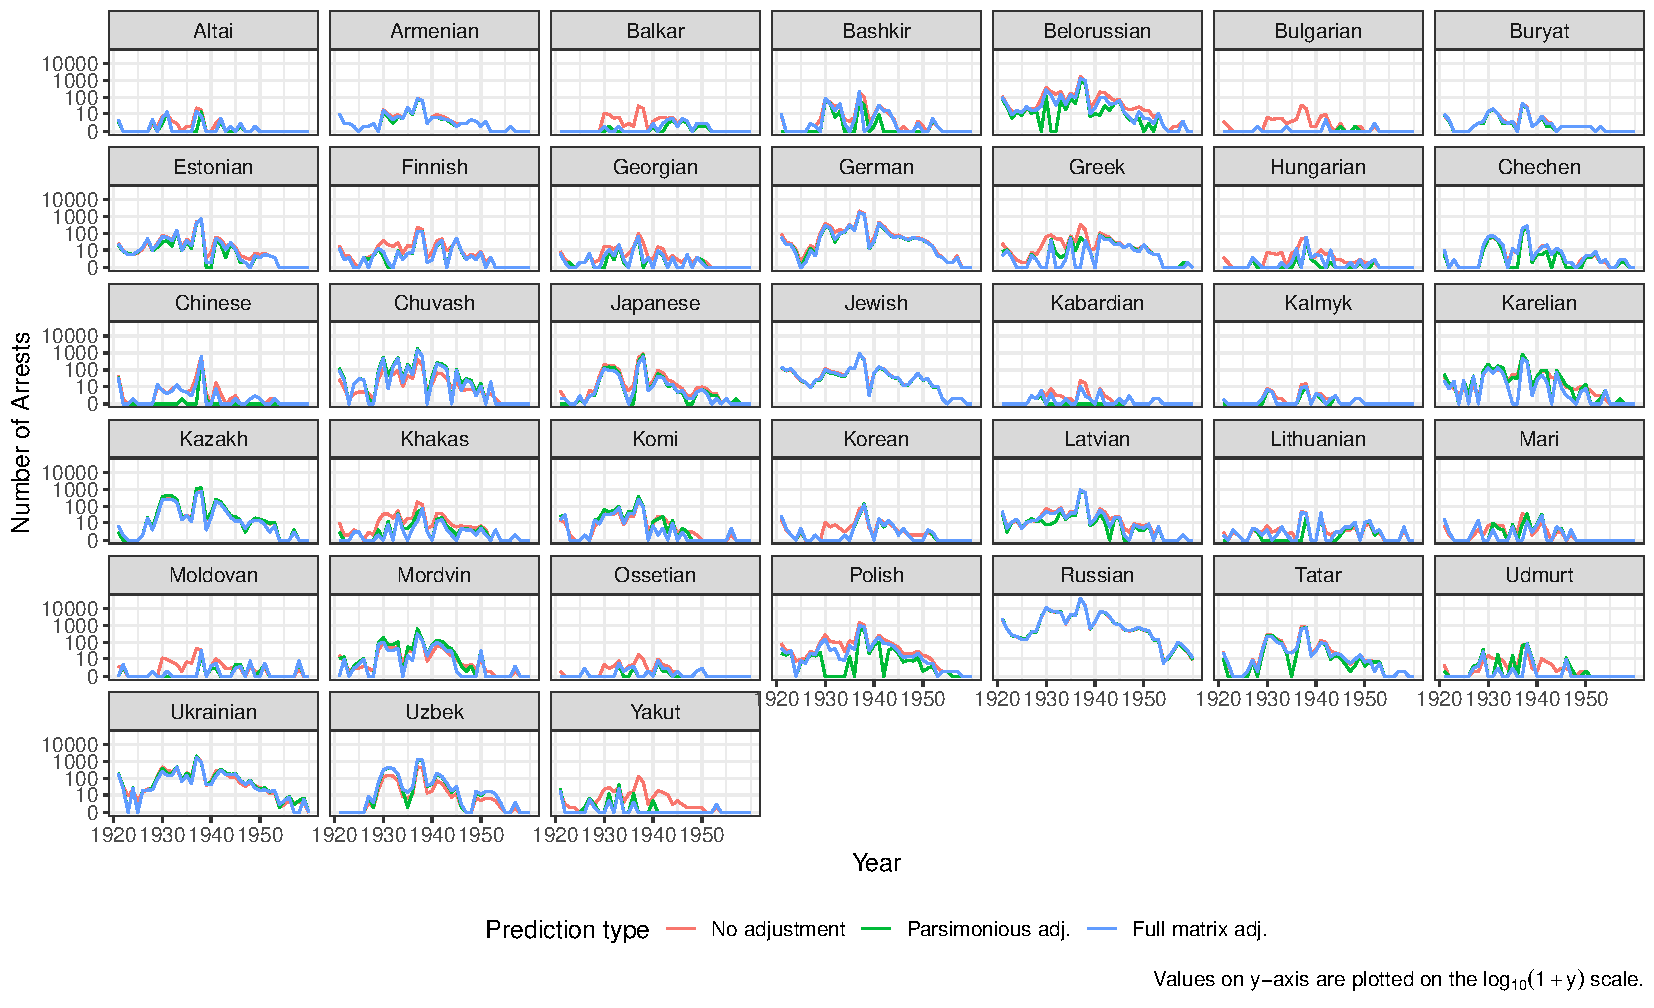
\includegraphics[width=1.2\textwidth]{plots/arrests/prediction_type_by_year.pdf}
\label{fig:prediction_type_by_year}
\end{figure}

\begin{figure}[H]
\centering
\caption{Histograms of Arrests by Ethnicity and Year}
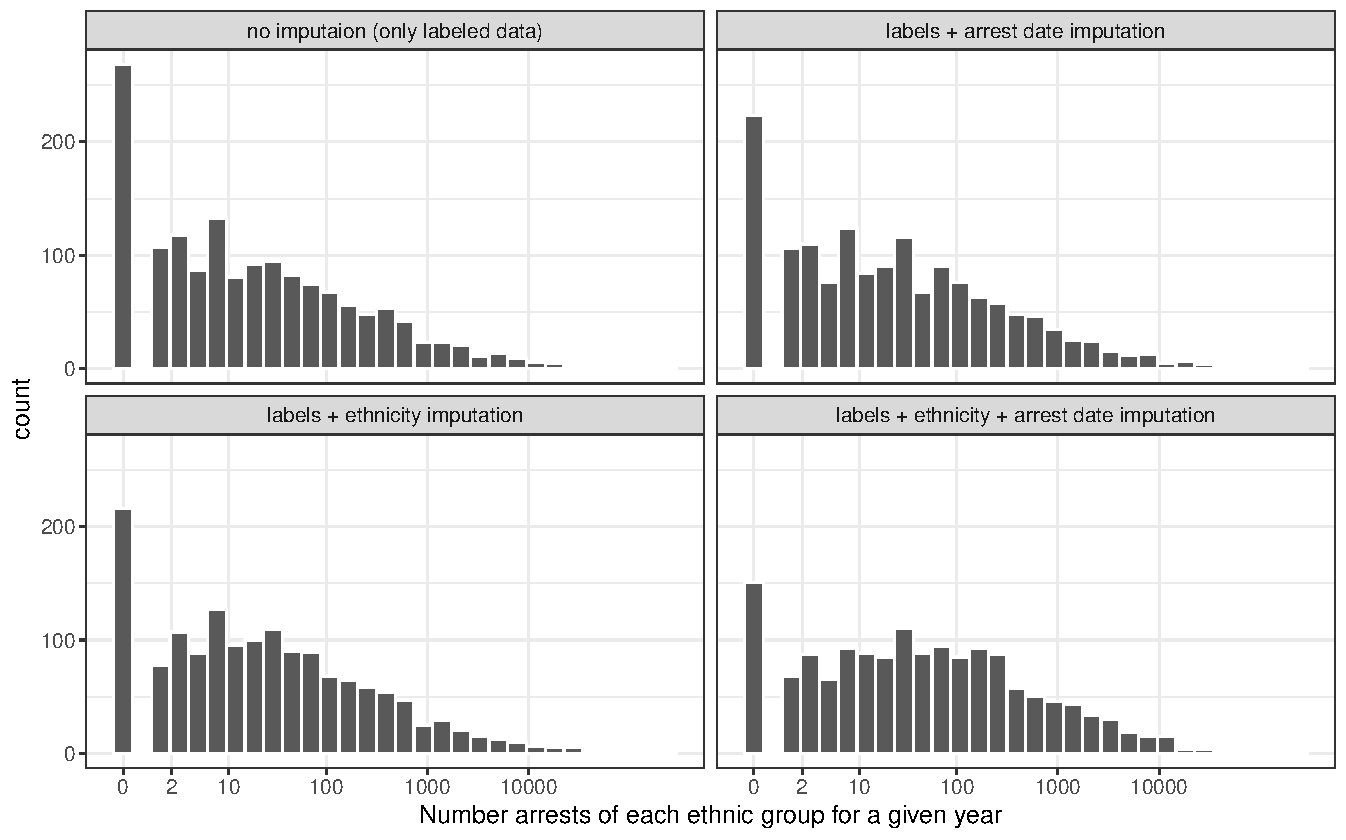
\includegraphics[width=1.2\textwidth]{plots/arrests/facet_hist.pdf}
\label{fig:facet_by_year}
\end{figure}

\begin{figure}[H]
\centering
\caption{Histogram of Imputed Number of Days between Arrest and Process}
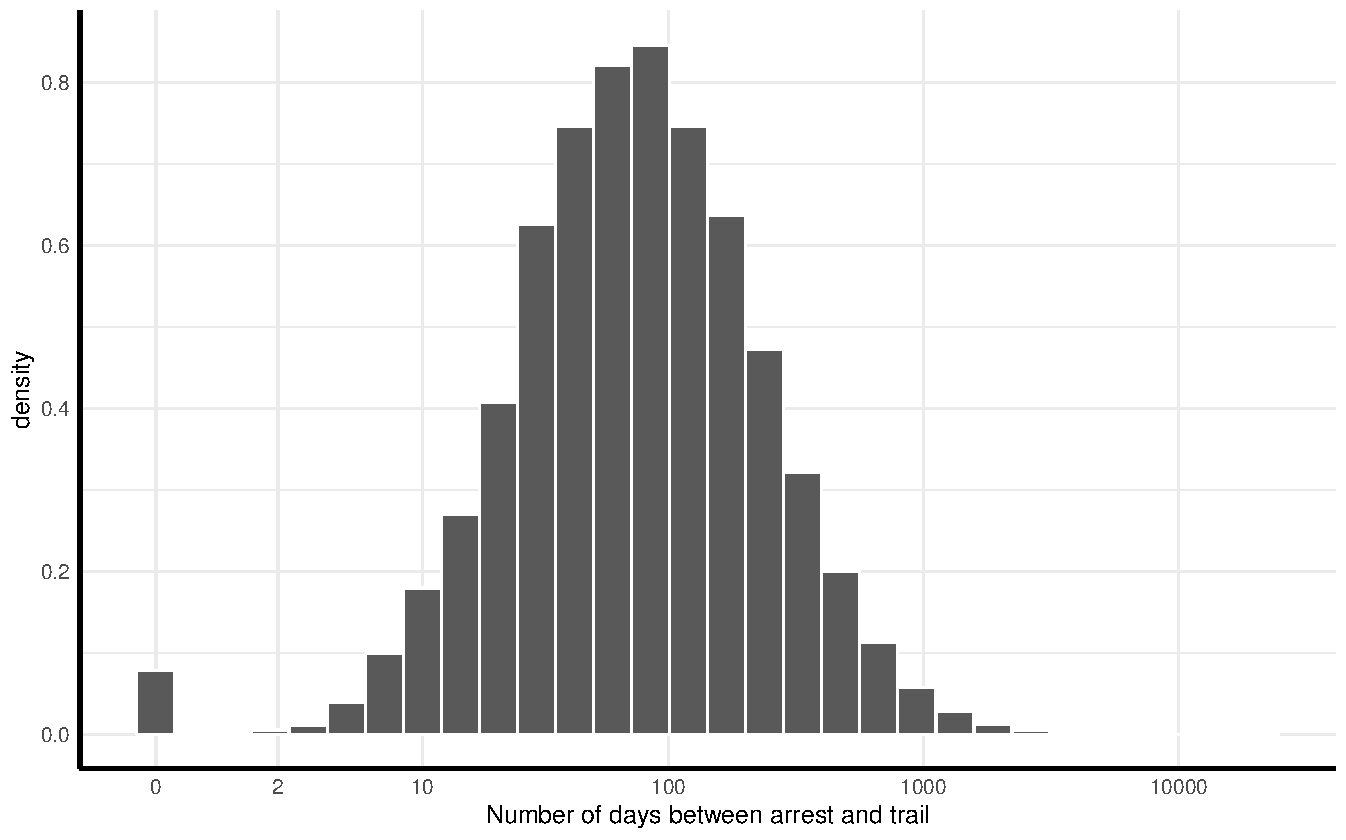
\includegraphics[width=1\textwidth]{plots/imputing_arrest_date/mixed_model_preds_hist.pdf}
\label{fig:mixed_model_preds_hist}
\end{figure}
\begin{figure}[H]
\caption{Time Series of Arrests }
\centering
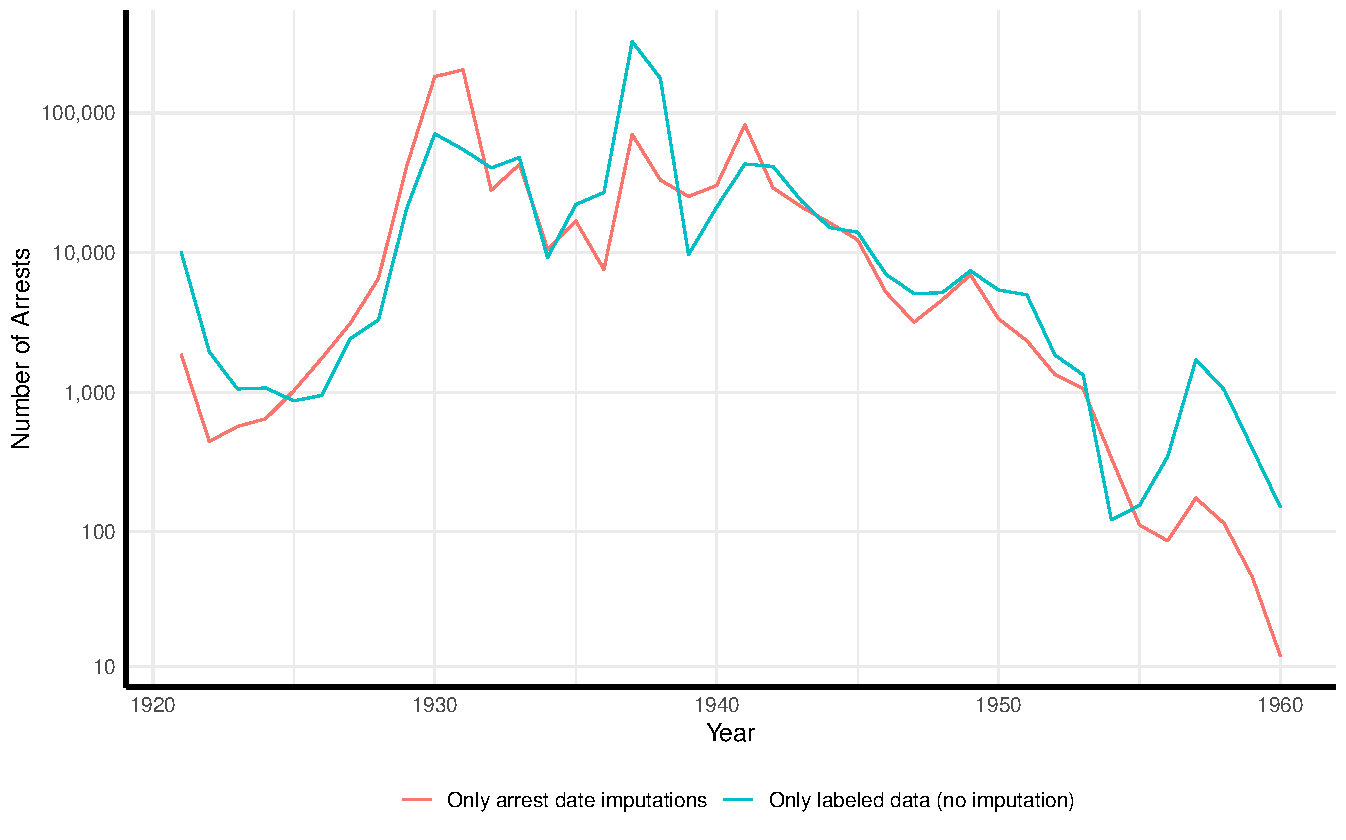
\includegraphics[width=\textwidth]{plots/arrests/date_imputation_line.pdf}
\label{fig:date_imputation_line}
\end{figure}


%\subsection{Difference-in-differnces Results}
 \begin{figure}[H]
\centering
\caption{Dynamic DiD, Only Ethnicities without Independent State}
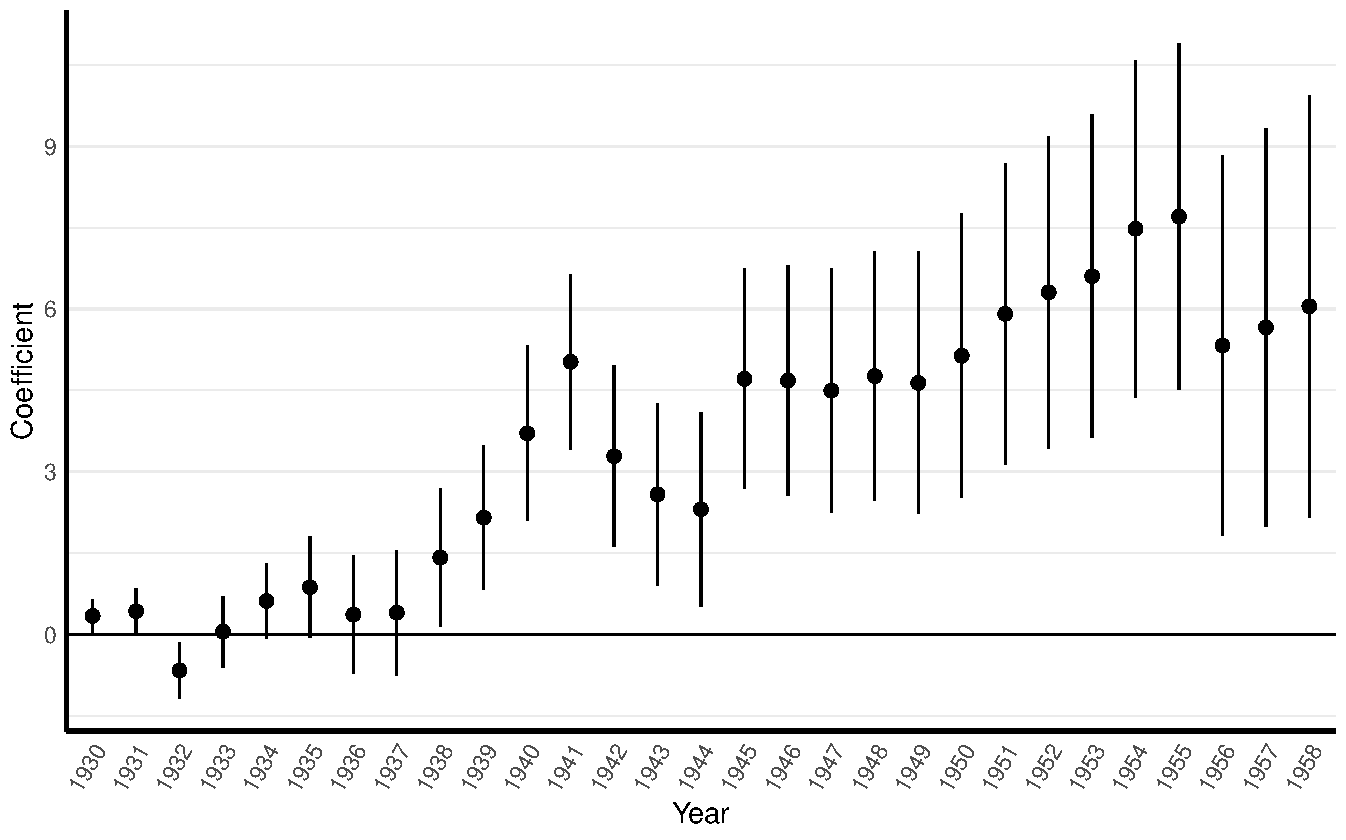
\includegraphics[width=\textwidth]{plots/effects/ethnicity_imputation/annual/pr_cr2_date_imp_full_years_not_ind_country.pdf}
\begin{minipage}{0.92\textwidth}
%\includegraphics[width=\linewidth]{Gaus.pdf}
%\rule{\linewidth}{10em}
\footnotesize
\emph{Notes:} Only ethnic groups without independent state are included in the control group. Ethnicity and date of arrest were imputed.  Full matrix adjustment was applied on ethnic group imputations. The quadratic ethnicity-specific time trends are included.  Standard errors are clustered on the level of ethnicity and are based on cluster robust estimator by \citet{pustejovsky_small-sample_2018}. Error bars show 95\% confidence intervals. 
\end{minipage}
\label{fig:did_effets_no_ind_countries}
\end{figure}

 \begin{figure}[H]
\centering
\caption{Dynamic DiD, Only Rehabilitated Individuals}
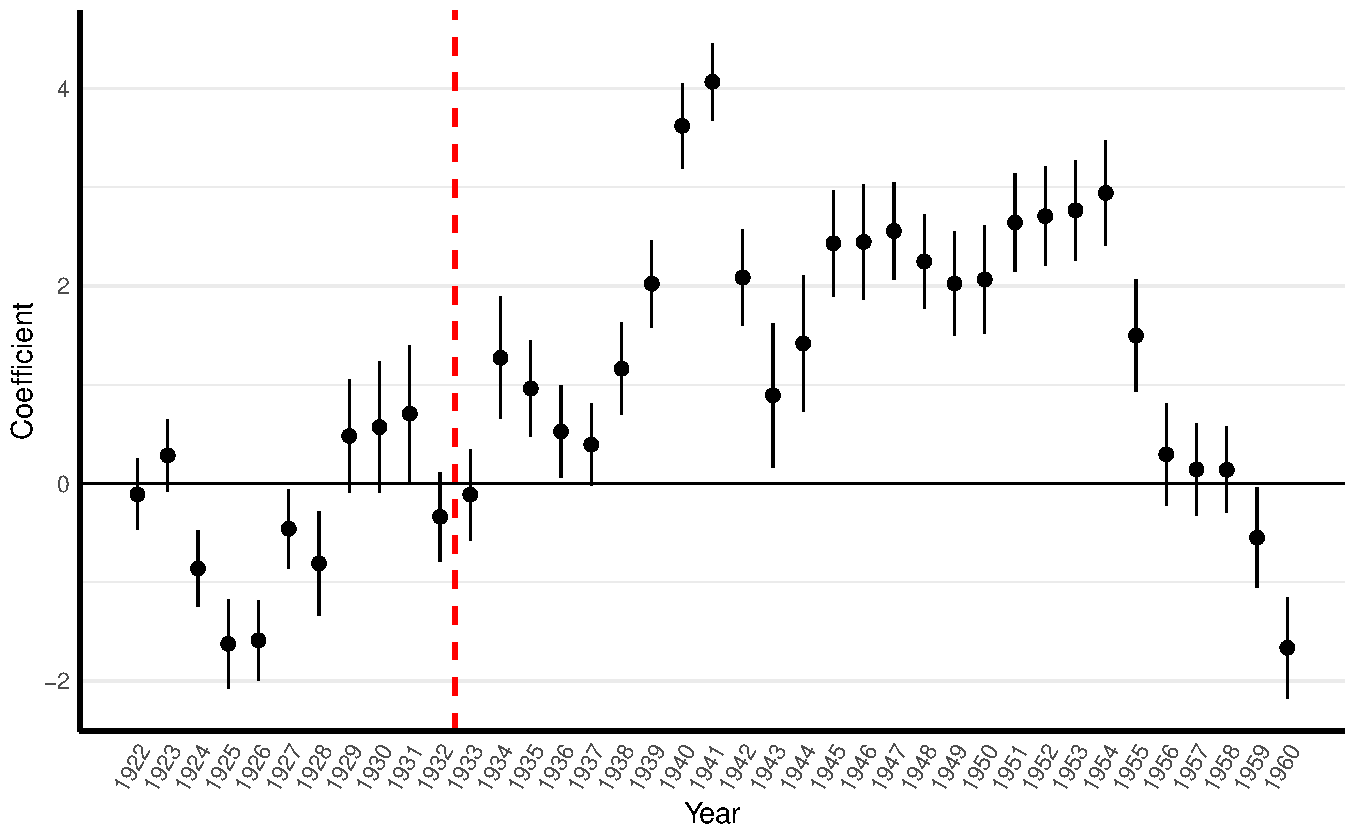
\includegraphics[width=\textwidth]{plots/final/fmla_pred_full_imp_date_no_trends_geopol_rehab_cr2.pdf}
\begin{minipage}{0.92\textwidth}
\footnotesize
\emph{Notes:} All 38 ethnic groups are included. Ethnicity and date of arrest were imputed.  Full matrix adjustment was applied on ethnic group imputations. Controls for major changes in relations with the USSR are included.
Standard errors are clustered on the level of ethnicity and are based on cluster robust estimator by \citet{pustejovsky_small-sample_2018}. Error bars show 95\% confidence intervals. 
\end{minipage}
\label{fig:did_effects_rehabs}
\end{figure}

 \begin{figure}[H]
\centering
\caption{Comparison of  Ethnicity-specific Time Trends for DiD}
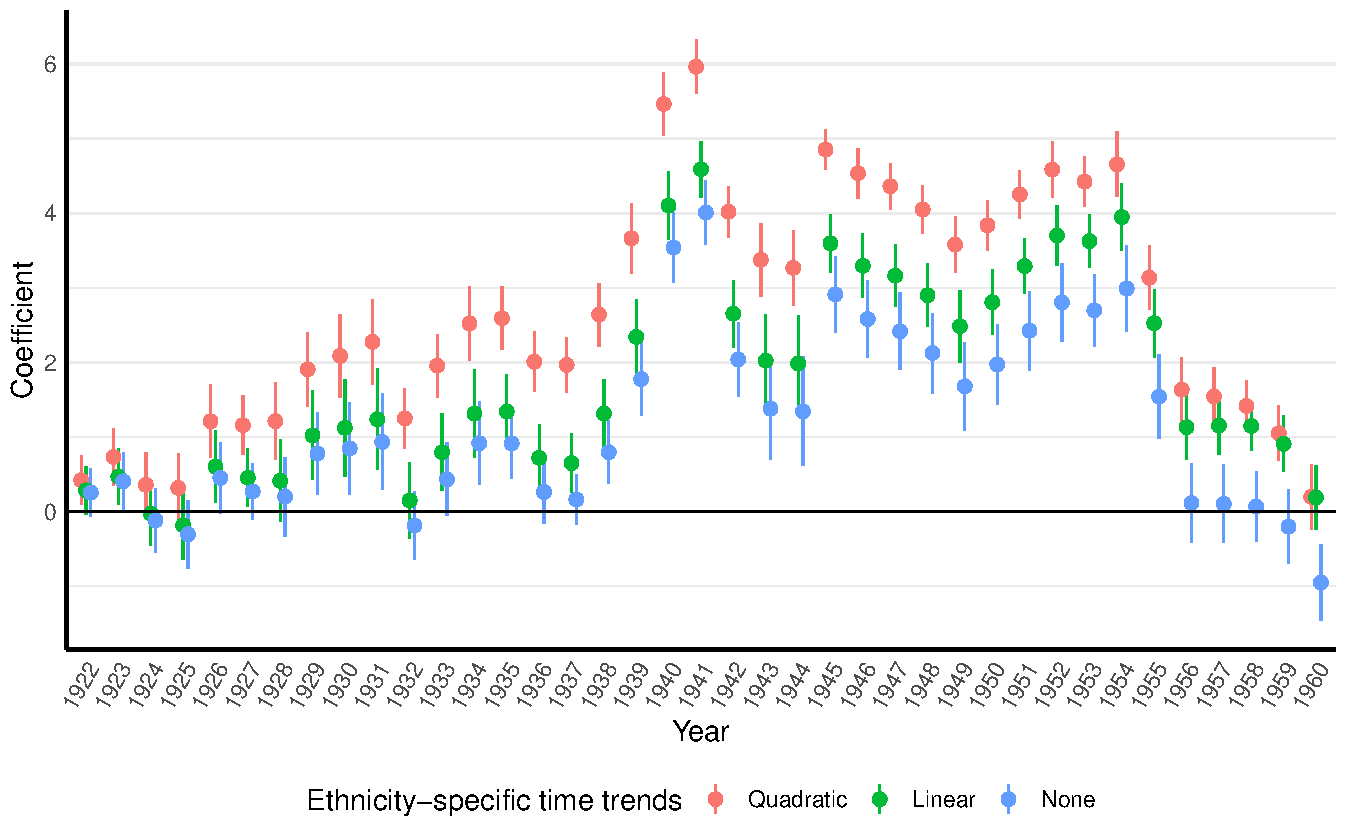
\includegraphics[width=\textwidth]{plots/effects/robustness_checks/trends_comp_pred_full_imp_date_cr2.pdf}
\begin{minipage}{\textwidth}
%\includegraphics[width=\linewidth]{Gaus.pdf}
%\rule{\linewidth}{10em}
\footnotesize
\emph{Notes:} All 38 ethnic groups are included. Ethnicity and date of arrest were imputed.  Full matrix adjustment was applied on ethnic group imputations.  Standard errors are clustered on the level of ethnicity and are based on cluster robust estimator by \citet{pustejovsky_small-sample_2018}. Error bars show 95\% confidence intervals. 
\end{minipage}
\label{fig:did_robustness_time_trends}
\end{figure}

 \begin{figure}[H]
\centering
\caption{Comparison of  Ethnicity Imputation Adjustments for DiD}
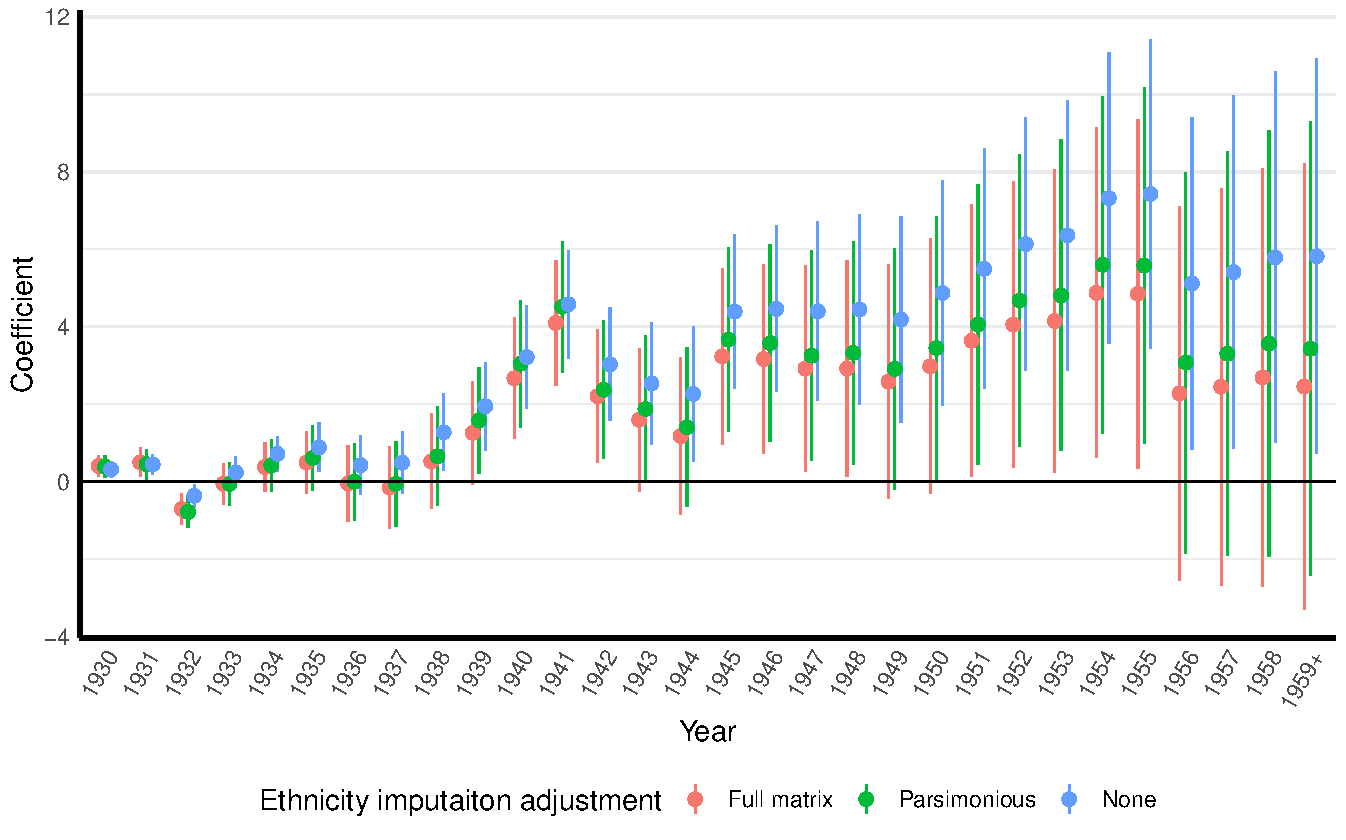
\includegraphics[width=\textwidth]{plots/effects/robustness_checks/pred_adj_comp_pred_full_imp_date_cr2.pdf}
\begin{minipage}{0.92\textwidth}
%\includegraphics[width=\linewidth]{Gaus.pdf}
%\rule{\linewidth}{10em}
\footnotesize
\emph{Notes:} All 38 ethnic groups are included. Ethnicity and date of arrest were imputed.   Standard errors are clustered on the level of ethnicity and are based on cluster robust estimator by \citet{pustejovsky_small-sample_2018}. Error bars show 95\% confidence intervals. 
\end{minipage}
\label{fig:did_robustness_pred_adj}
\end{figure}


%
% Table created by stargazer v.5.2.2 by Marek Hlavac, Harvard University. E-mail: hlavac at fas.harvard.edu
% Date and time: p�, led 11, 2019 - 10:10:43
\begin{table}[!htbp] \centering 
  \caption{Difference-in-differences results} 
  \label{dif_table} 
\begin{tabular}{@{\extracolsep{5pt}}lcccc} 
\\[-1.8ex]\hline 
\hline \\[-1.8ex] 
 & \multicolumn{4}{c}{\textit{Dependent variable:}} \\ 
\cline{2-5} 
\\[-1.8ex] & \multicolumn{3}{c}{$\log(1 + y_{it})$} & $y_{it}$ \\ 
 & 1921-1958 & 1921-1945 & 1921-1945 & 1921-1958 \\ 
\\[-1.8ex] & (1) & (2) & (3) & (4)\\ 
\hline \\[-1.8ex] 
 $german*post\_1930$ & 1.196 & 0.731 & 0.855 & 683.539 \\ 
  & (0.887) & (0.984) & (0.963) & (1,495.164) \\ 
  & & & & \\ 
 $german*post\_1931$ & $-$0.779 & $-$0.872 & $-$0.847 & $-$61.209 \\ 
  & (1.177) & (1.198) & (1.292) & (1,983.046) \\ 
  & & & & \\ 
 $german*post\_1932$ & $-$0.439 & $-$0.532 & $-$0.507 & 63.854 \\ 
  & (1.177) & (1.198) & (1.292) & (1,983.046) \\ 
  & & & & \\ 
 $german*post\_1933$ & 0.365 & 0.272 & 0.297 & 199.791 \\ 
  & (1.177) & (1.198) & (1.292) & (1,983.046) \\ 
  & & & & \\ 
 $german*post\_1934$ & 2.040$^{*}$ & 1.947 & 1.971 & 996.604 \\ 
  & (1.177) & (1.198) & (1.292) & (1,983.046) \\ 
  & & & & \\ 
 $german*post\_1935$ & $-$0.638 & $-$0.731 & $-$0.706 & 49.979 \\ 
  & (1.177) & (1.198) & (1.292) & (1,983.046) \\ 
  & & & & \\ 
 $german*post\_1936$ & $-$0.134 & $-$0.227 & $-$0.202 & 71.041 \\ 
  & (1.177) & (1.198) & (1.292) & (1,983.046) \\ 
  & & & & \\ 
 $german*post\_1937$ & $-$0.214 & $-$0.307 & $-$0.282 & 637.291 \\ 
  & (1.177) & (1.198) & (1.292) & (1,983.046) \\ 
  & & & & \\ 
 $german*post\_1938$ & 1.322 & 0.772 & 0.537 & 2,304.034 \\ 
  & (0.906) & (0.972) & (0.934) & (1,526.238) \\ 
  & & & & \\ 
\hline \\[-1.8ex] 
Year dummies & Yes & Yes & Yes & Yes \\ 
Ethnicity dummies & Yes & Yes & Yes & Yes \\ 
Ethnicity time trends & Yes & Yes & No & Yes \\ 
Observations & 663 & 425 & 663 & 663 \\ 
R$^{2}$ & 0.890 & 0.900 & 0.864 & 0.428 \\ 
Adjusted R$^{2}$ & 0.875 & 0.882 & 0.850 & 0.350 \\ 
\hline 
\hline \\[-1.8ex] 
\textit{Note:}  & \multicolumn{4}{r}{$^{*}$p$<$0.1; $^{**}$p$<$0.05; $^{***}$p$<$0.01} \\ 
\end{tabular} 
\end{table} 

%\thispagestyle{empty}

\begin{figure}[H] 
\caption{Gaps between synthetic control and actual values for placebo tests}
\begin{subfigure}{\textwidth}
\caption{All ethnic groups}
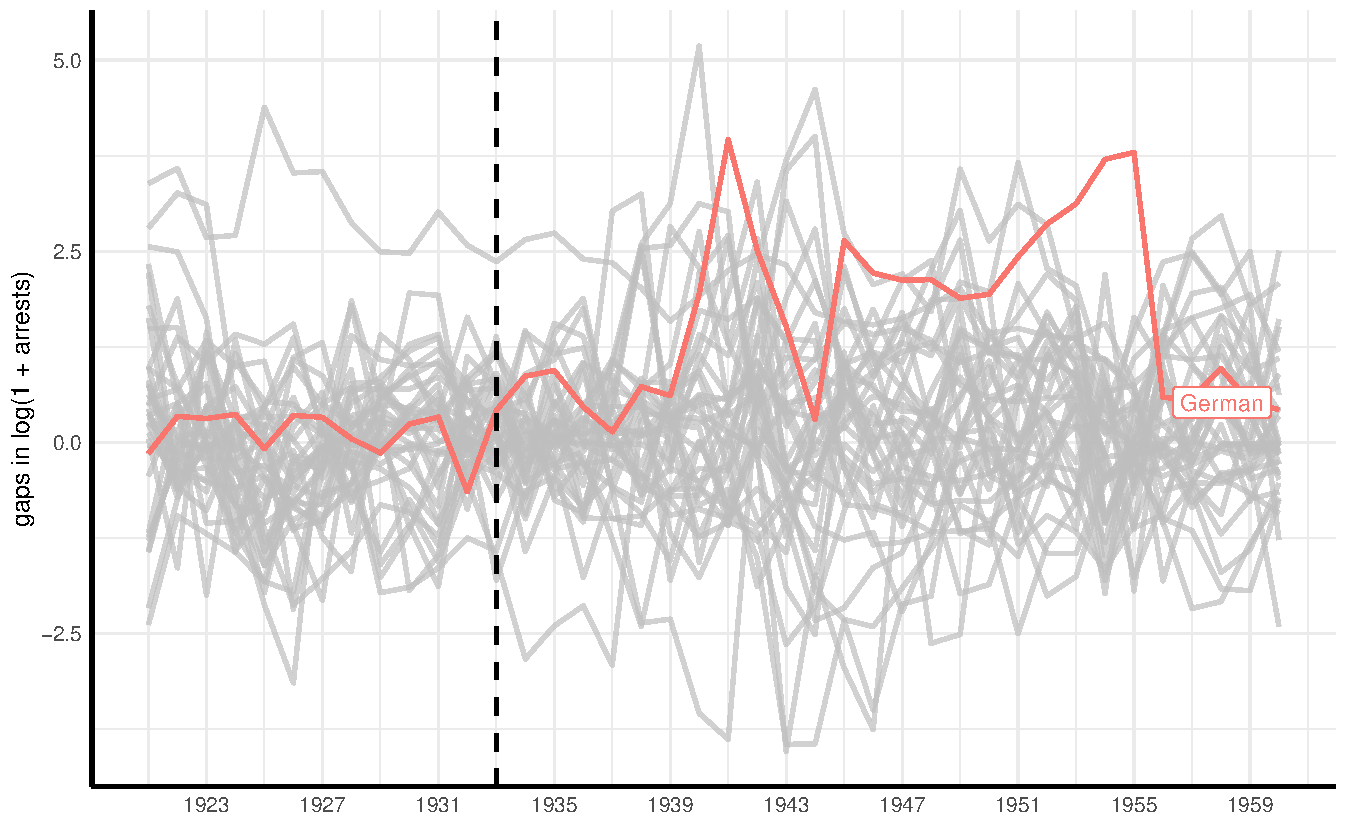
\includegraphics[width=0.9\linewidth]{plots/synthetic_control/ethnicity_imputation/annual/placebo_highlight_all_imp_date_robustnes.pdf}
\label{fig:sc_placebo_gaps_all_robutness}
\end{subfigure}
\begin{subfigure}{\textwidth}
\caption{Ethnic groups with pre-treatment MSPE higher than 20 times the MSPE of Germans excluded}
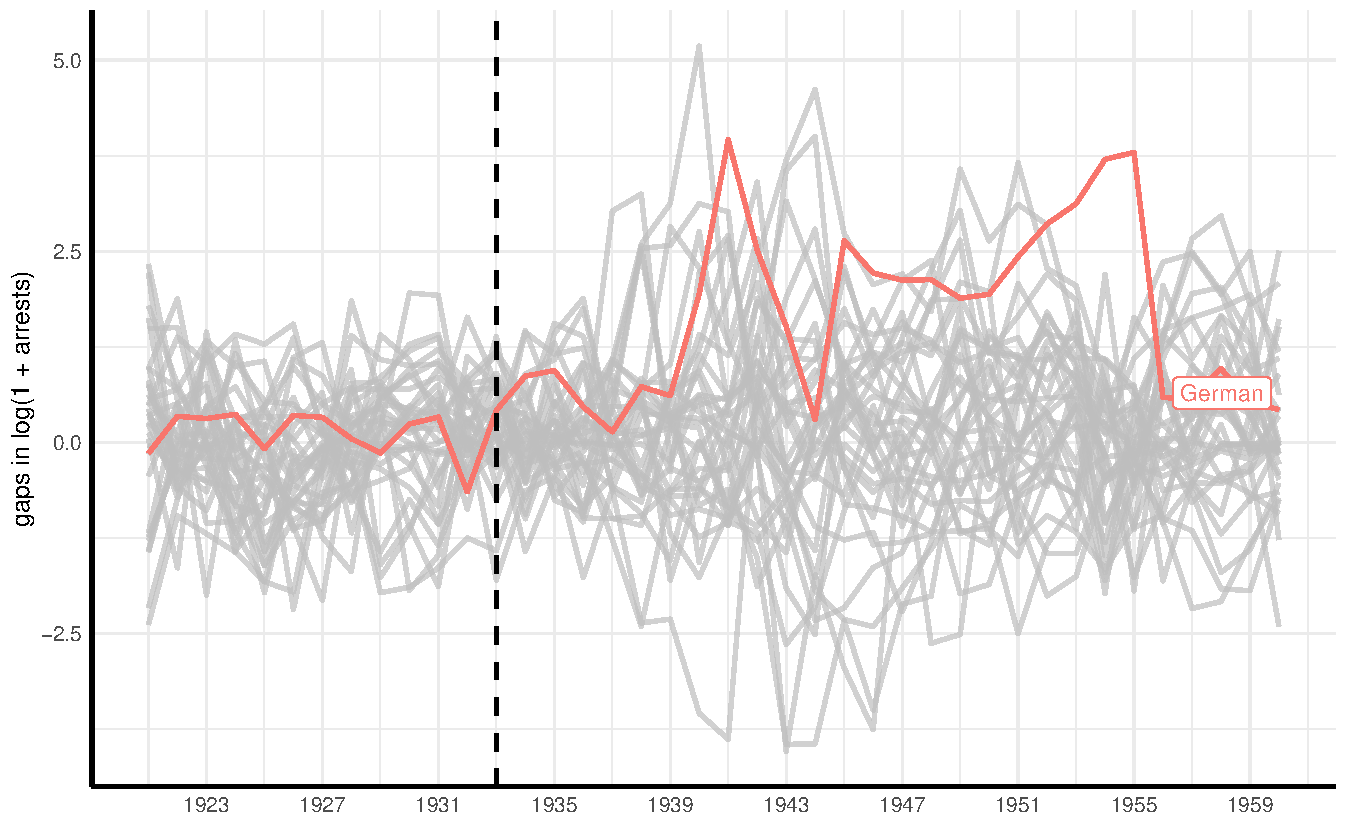
\includegraphics[width=0.9\linewidth]{plots/synthetic_control/ethnicity_imputation/annual/placebo_highlight_mspe_20lower_imp_date_robustnss.pdf}
%Ethnic groups with pre-treatment MSPE higher than 5 times the MSPE of Germany excluded
\label{fig:sc_placebo_gaps_all_20_times_robustness}
\end{subfigure}
\label{fig:sc_placebo_gaps_robustness}
\begin{minipage}{0.92\textwidth}
\footnotesize
\emph{Notes:} The predictors are the mean of $\log\left(1 + \text{arrests}\right)$ in the pre-treatment period, total population of the ethnic group in the USSR and its urbanization rate (both taken from the 1926 Soviet census), and linguistic similarity to Russian.  Ethnicity and date of arrest were imputed.  Full matrix adjustment was applied on ethnic group imputations. All 38 ethnic groups are included. 
\end{minipage}
\end{figure}


\begin{figure}[H] 
\caption{Ratios of post-treatment MSPE to pre-treatment MSPE}
\begin{subfigure}{\textwidth}
\caption{The whole post-treatment period in the numerator (1933-1960)}
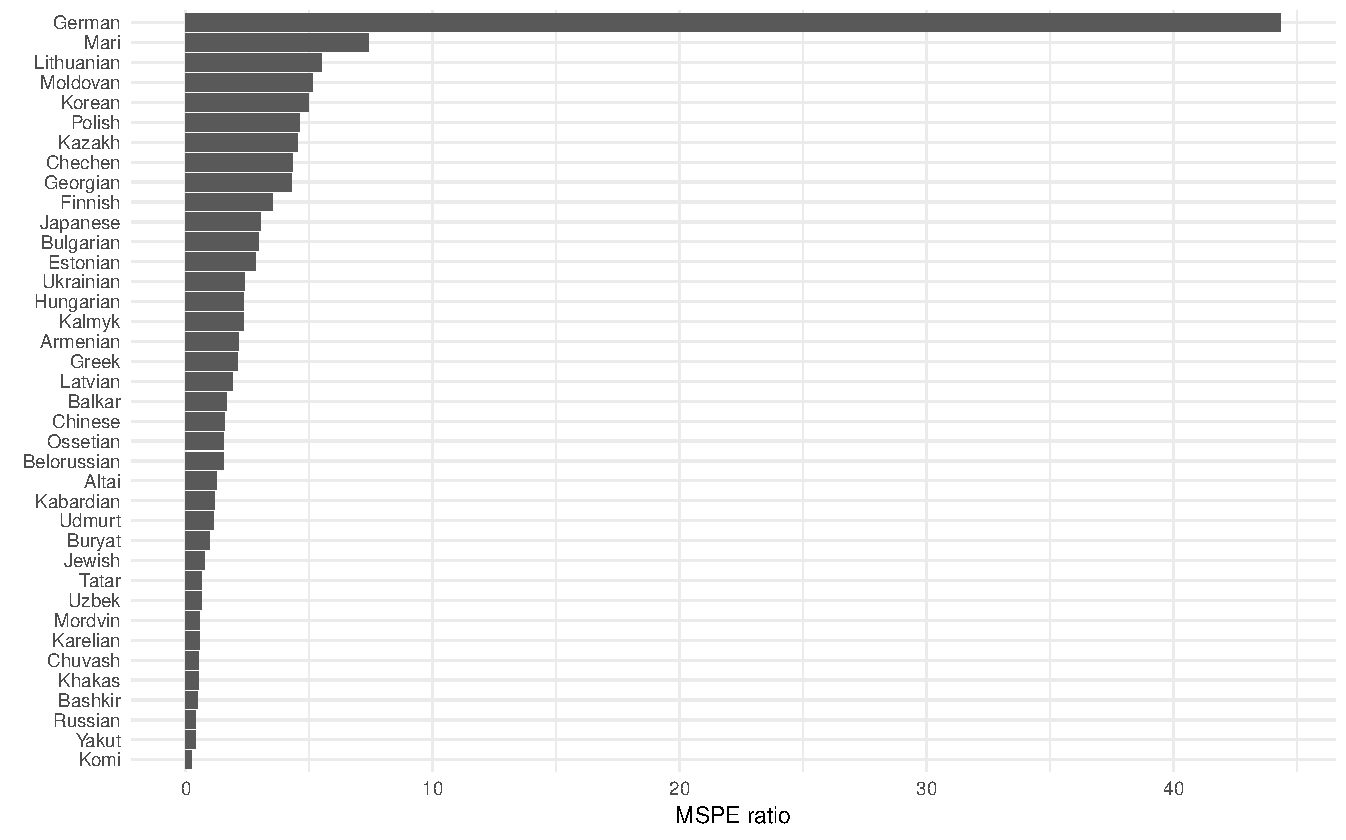
\includegraphics[width=\linewidth]{plots/synthetic_control/ethnicity_imputation/annual/mspe_ratios_imp_date_robustness.pdf}
\label{fig:sc_mspe_ratios_all_robustness}
\end{subfigure}
\begin{subfigure}{\textwidth}
\caption{Only the period from 1933 to 1939 in the numerator}
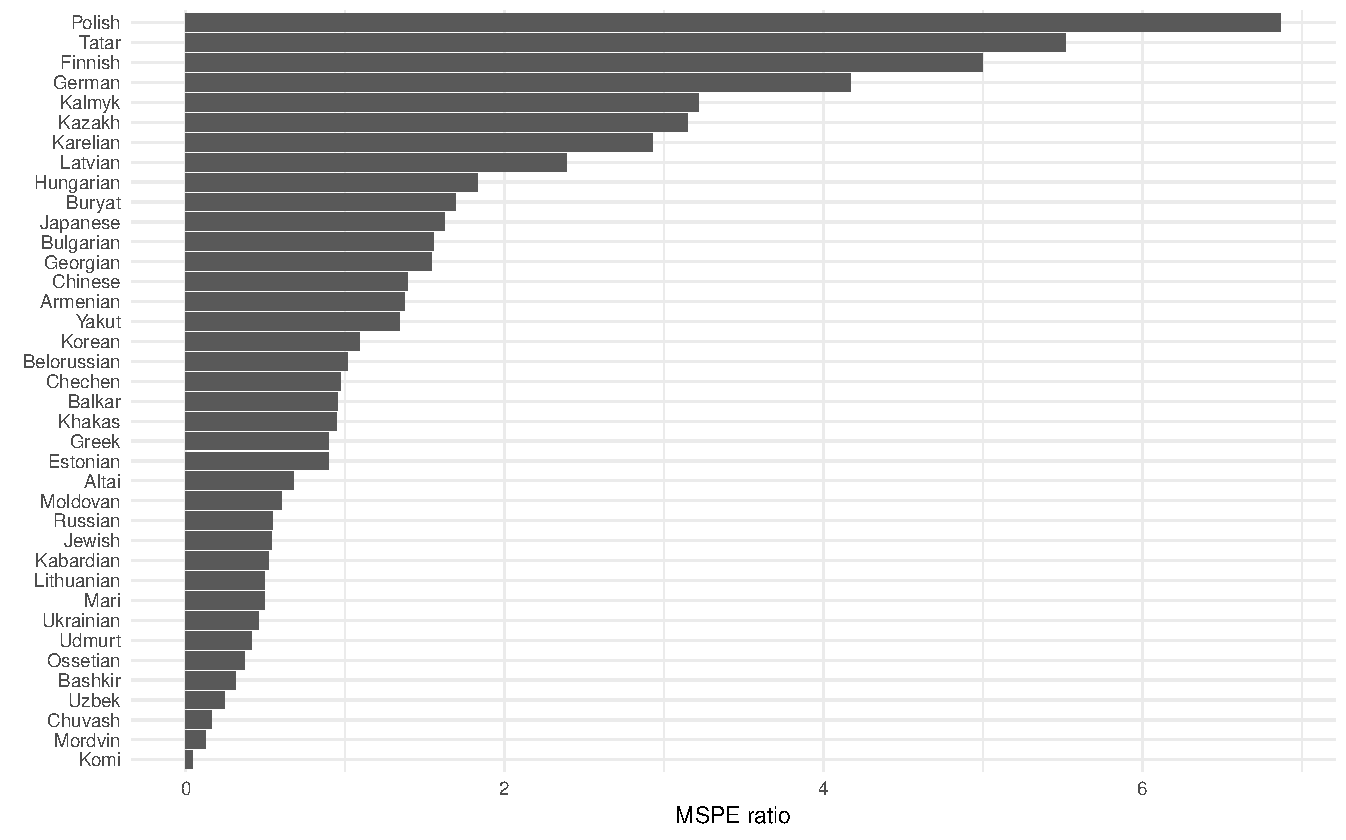
\includegraphics[width=\linewidth]{plots/synthetic_control/ethnicity_imputation/annual/mspe_ratios_imp_date_until_1939_robustness.pdf}
%Ethnic groups with pre-treatment MSPE higher than 5 times the MSPE of Germany excluded
\label{fig:sc_mspe_ratios_until_1939_robustness}
\end{subfigure}
\label{fig:sc_mspe_ratios_robustness}
\begin{minipage}{0.92\textwidth}
\footnotesize
\emph{Notes:} The same as for the figure \ref{fig:sc_placebo_gaps_robustness}.
\end{minipage}
\end{figure}



\begin{figure}[H] 
\caption{Gaps between synthetic control and actual values for placebo tests}
\begin{subfigure}{\textwidth}
\caption{Only ethnicities without independent state}
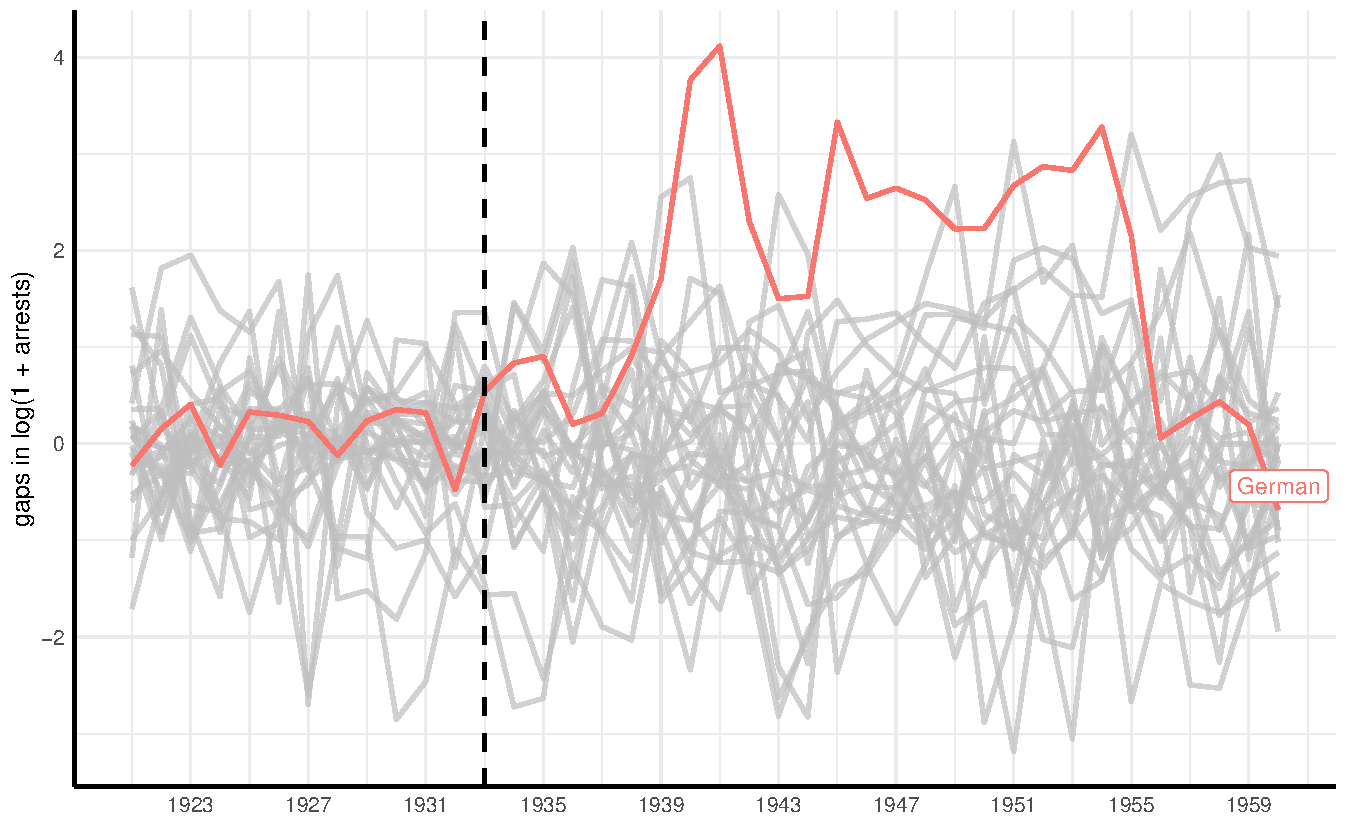
\includegraphics[width=0.9\linewidth]{plots/final/placebo_highlight_all_ethnicities_without_ind_state.pdf}
\label{fig:sc_placebo_gaps_all_without_ind_state}
\end{subfigure}
\begin{subfigure}{\textwidth}
\caption{Only rehabilitated individuals}
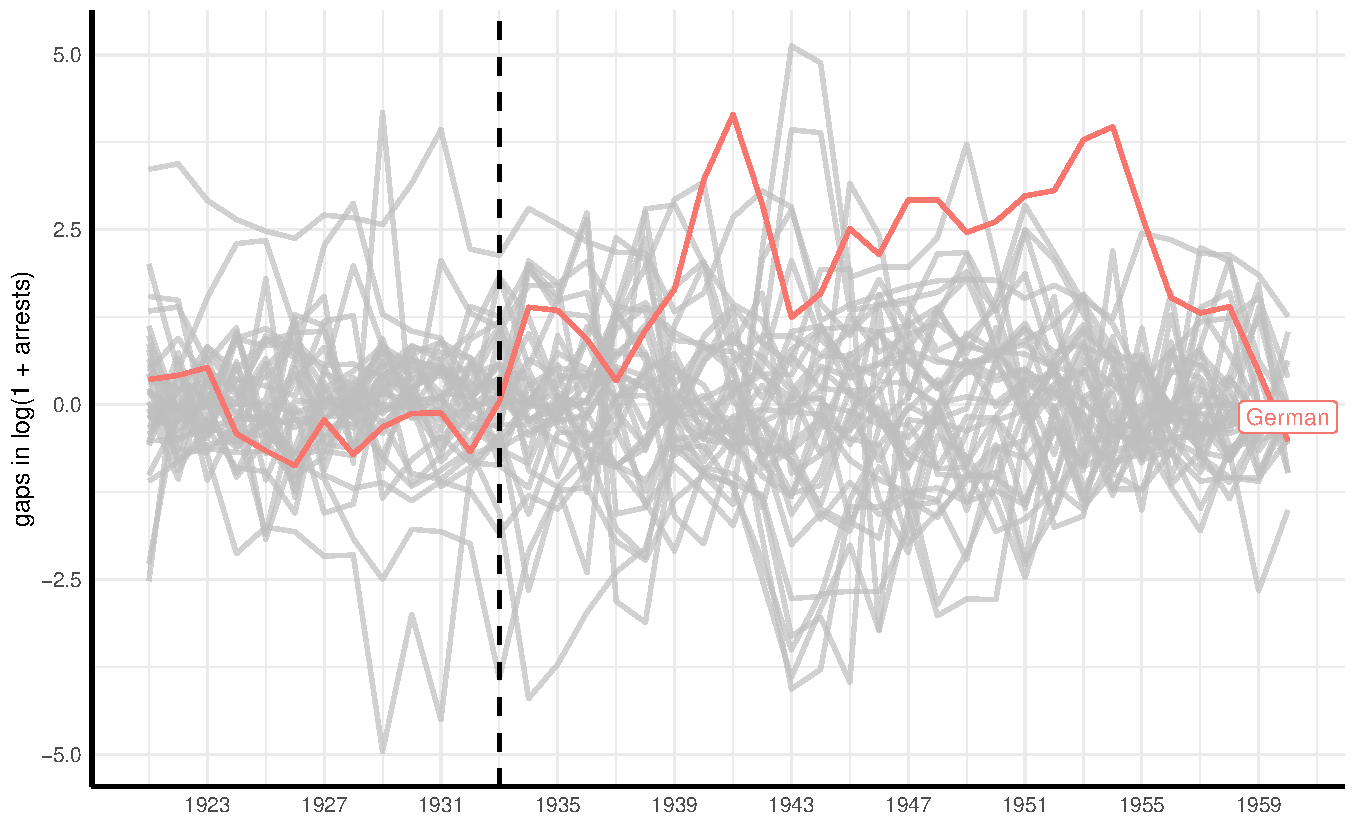
\includegraphics[width=0.9\linewidth]{plots/final/placebo_highlight_all_rehabs.pdf}
%Ethnic groups with pre-treatment MSPE higher than 5 times the MSPE of Germany excluded
\label{fig:sc_placebo_gaps_all_rehabs}
\end{subfigure}
\label{fig:sc_placebo_gaps_more_rob_checks}
\begin{minipage}{0.92\textwidth}
\footnotesize
\emph{Notes:} 
All pre-treatment outcomes were used as predictors. 
%The predictors are the mean of $\log\left(1 + \text{arrests}\right)$ in the pre-treatment period, total population of the ethnic group in the USSR and its urbanization rate (both taken from the 1926 Soviet census), and linguistic similarity to Russian.
Ethnicity and date of arrest were imputed.  Full matrix adjustment was applied on ethnic group imputations.
\end{minipage}
\end{figure}

\begin{figure}[H] 
\caption{Ratios of post-treatment MSPE to pre-treatment MSPE}
\begin{subfigure}{\textwidth}
\caption{Only ethnicities without independent state}
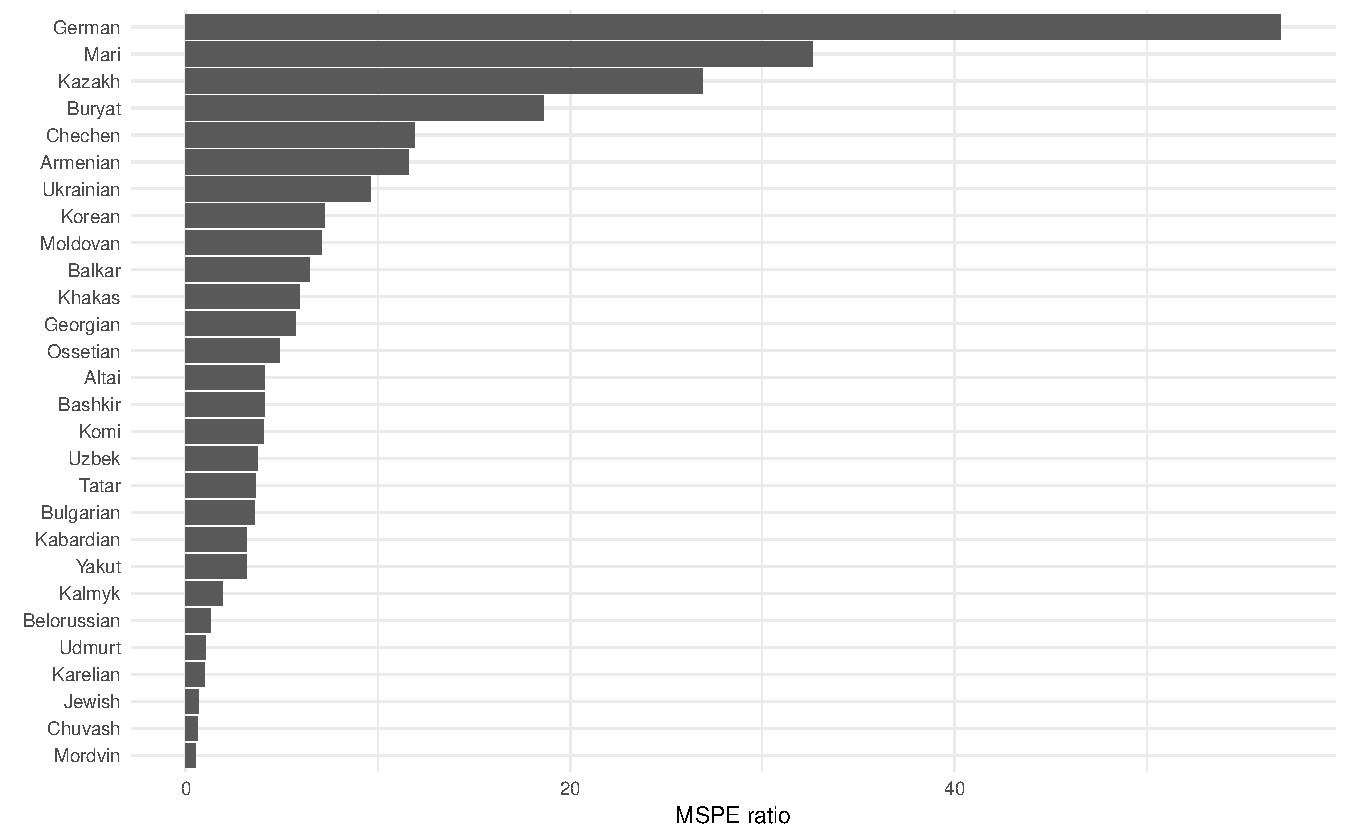
\includegraphics[width=\linewidth]{plots/final/mspe_ratios_ethnicities_without_ind_state.pdf}
\label{fig:sc_mspe_ratios_without_ind_state}
\end{subfigure}
\begin{subfigure}{\textwidth}
\caption{Only rehabilitated individuals}
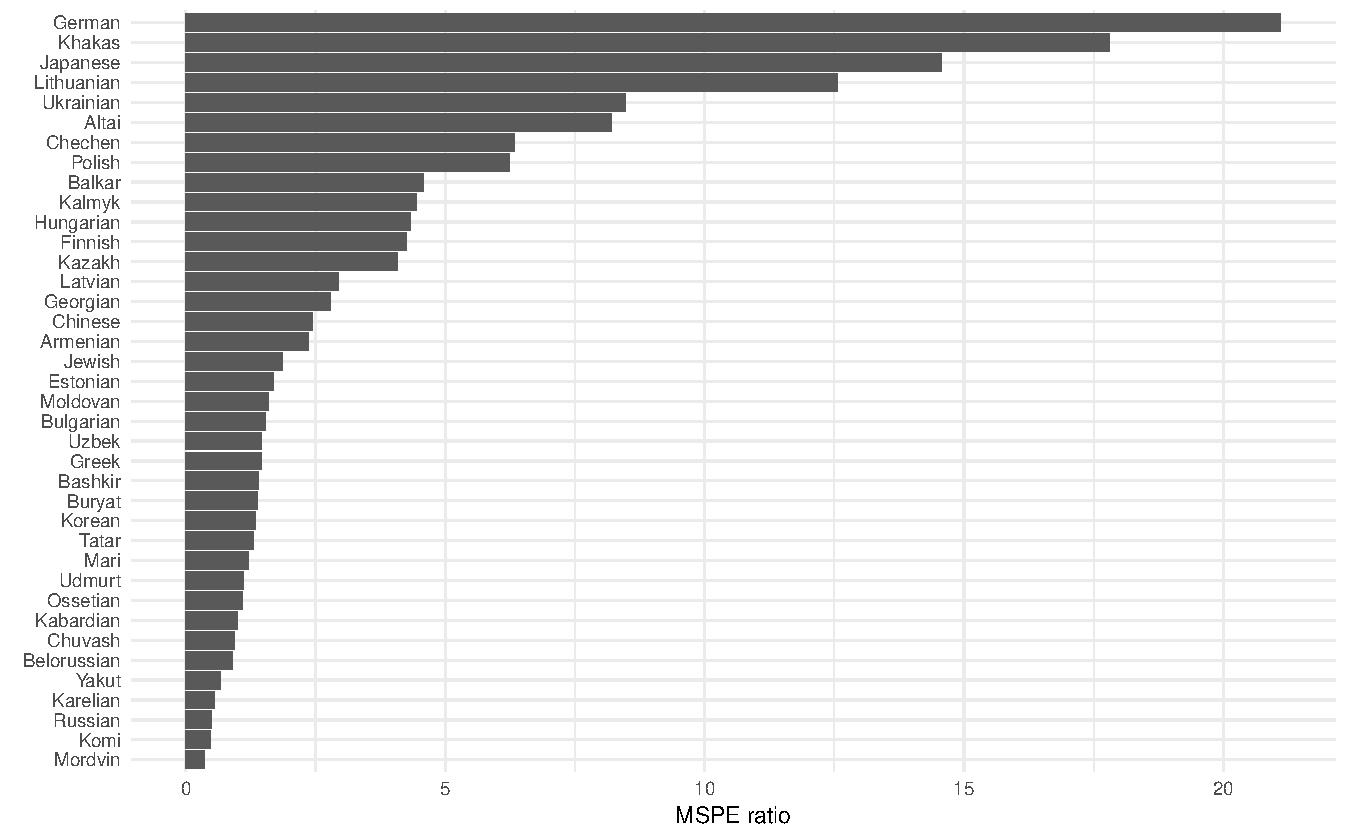
\includegraphics[width=\linewidth]{plots/final/mspe_ratios_rehabs.pdf}
%Ethnic groups with pre-treatment MSPE higher than 5 times the MSPE of Germany excluded
\label{fig:sc_mspe_ratios_rehabs}
\end{subfigure}
\label{fig:sc_mspe_ratios_more_rob_checks}
\begin{minipage}{0.92\textwidth}
\footnotesize
\emph{Notes:} The whole post-treatment period in the numerator (1933-1960) for both figures.  Otherwise same as for the figure \ref{fig:sc_placebo_gaps_more_rob_checks}.
\end{minipage}
\end{figure}